% !TeX root = ./report.tex

\documentclass{IEEEtran}
\usepackage{bm}
\usepackage{amsmath}
\usepackage{amssymb}
\usepackage{booktabs}
\usepackage{algorithm}
\usepackage{algorithmicx}
\usepackage{algpseudocode}
\usepackage{footnote}
\usepackage{stfloats}
\usepackage{graphicx}
\usepackage{url}
\DeclareMathOperator*{\argmax}{arg\,max}
\DeclareMathOperator*{\argmin}{arg\,min}
\makesavenoteenv{figure}
\title{Title}
\author{
    Fan~JIN
    \thanks{Fan~JIN 2015011506  \texttt{jinf15@mails.tsinghua.edu.cn}}
}

\begin{document}
\maketitle
\begin{abstract}
    Abstract
\end{abstract}
\begin{IEEEkeywords}
    Keywords 1, Keywords 2,
\end{IEEEkeywords}

\section{Question 1: Function Optimization}
{
    \subsection{Target function: Eggholder}
    {
        As intelligent optimization algorithms have emerged as a new paradigm of function optimization, 
        many test functions have been proposed to serve as benchmarks \cite{wiki:Test_functions_for_optimization}.
        In this report, the Eggholder function is chosen to test two intelligent optimization algorithms:
        the simulated annealing (SA) and the differential evolution (DE).

        The Eggholder function is defined as
        \[
            \begin{split}
            f(x,y) &= \\
            &- (y+47) \sin{\sqrt{\left| \frac{x}{2}+(y+47) \right|}} \\
            &- x \sin{\sqrt{\left| x-(y+47) \right|}},
            \end{split}
        \]
        where $-512 < x,y < 512$.
        Its global minimum is known as $f(512, 404.2319) = -959.6407$. (Figure \ref{fig:eggholder})

        \begin{figure}[!htbp]
            \centering
            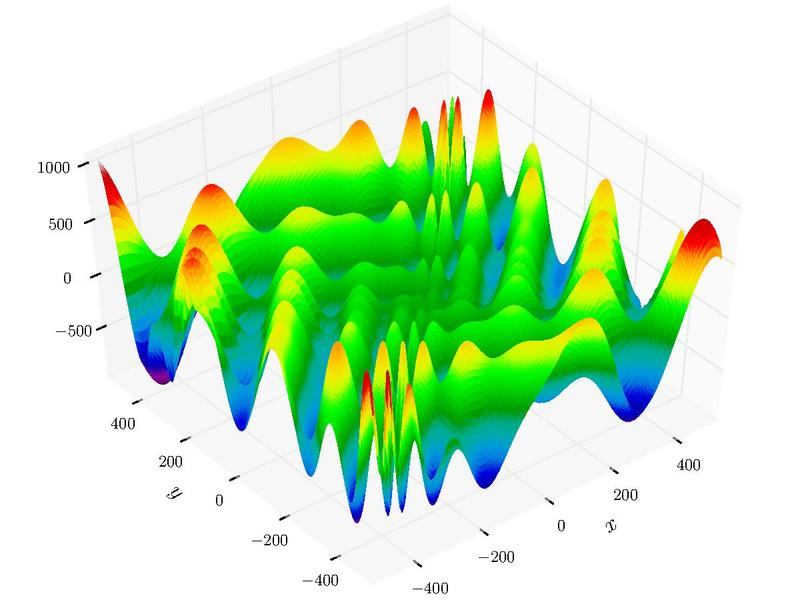
\includegraphics[width=0.45\textwidth]{figures/eggholder.png}
            \caption{Eggholder function \cite{wiki:Test_functions_for_optimization}}
            \label{fig:eggholder}
        \end{figure}

        Eggholder function is challenging bacause 
        i) it has boundary constraints on both $x$ and $y$, and 
        ii) the global minimum is at the boundary of $x=512$, and 
        iii) there are dozens of local minimums throughout the space.
        
    }

    \subsection{Implementation of SA and DE}
    {
        \begin{figure}[!htbp]
            \centering
            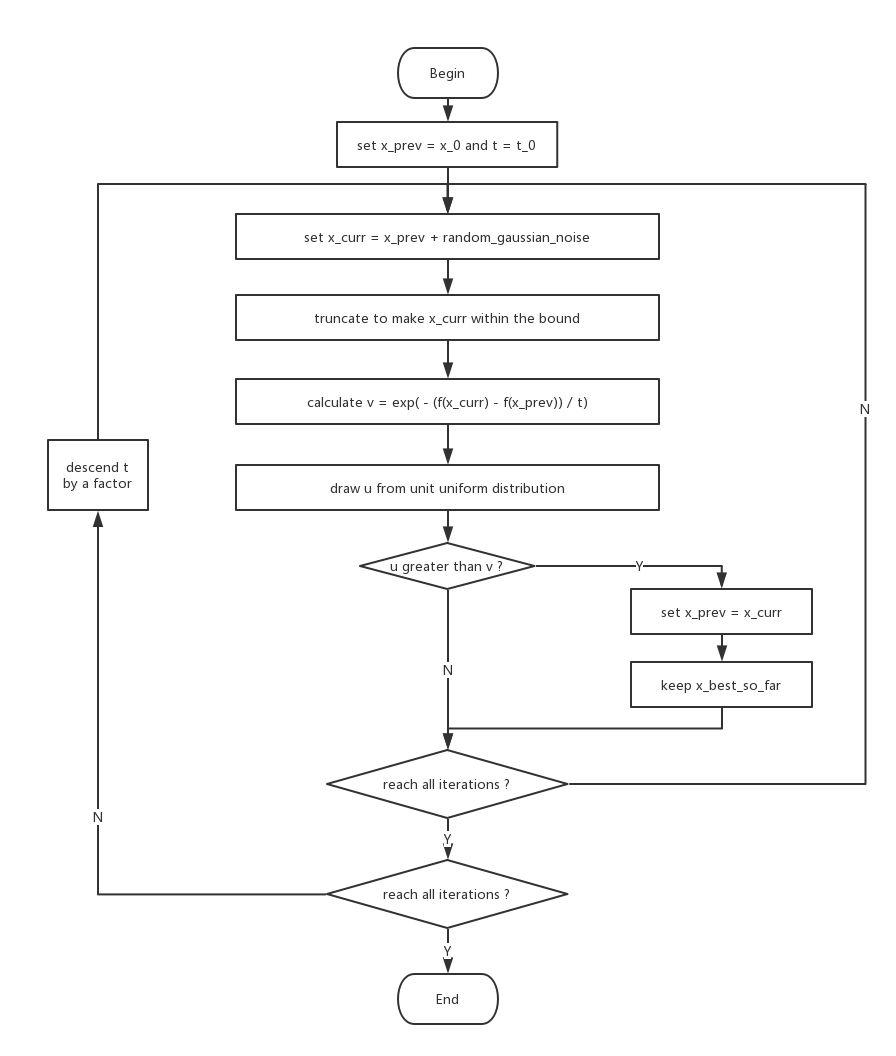
\includegraphics[width=0.45\textwidth]{figures/SA_algorithm.png}
            \caption{Flow chart of simulated annealing (SA)}
            \label{fig:SA}
        \end{figure}

        \begin{figure}[!htbp]
            \centering
            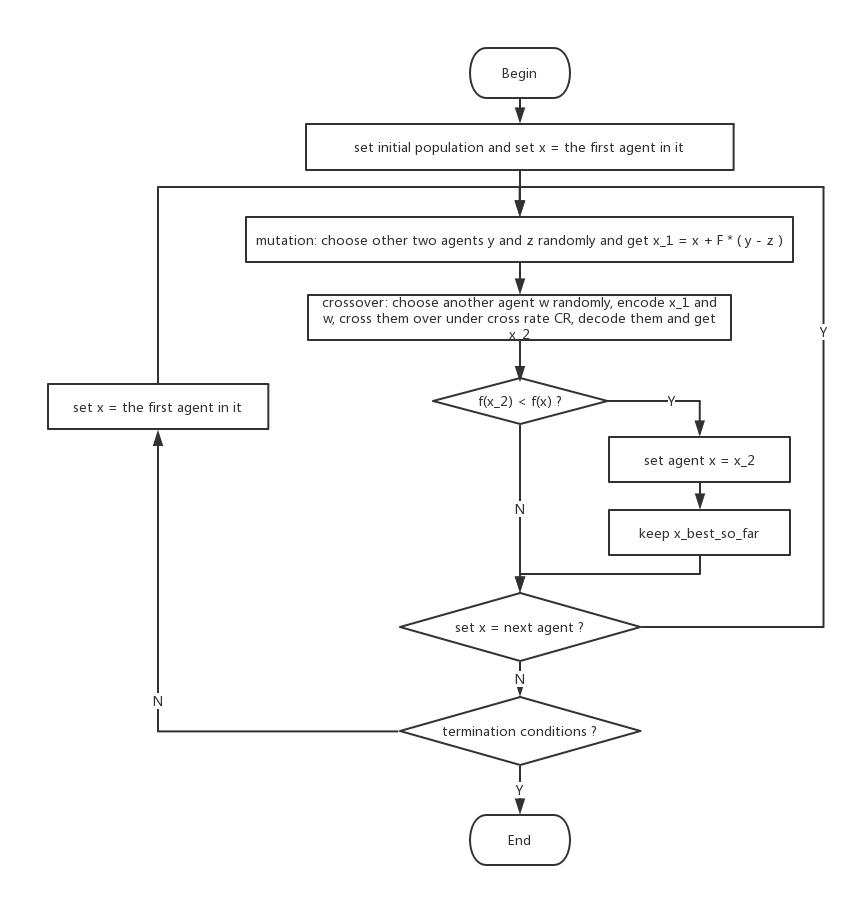
\includegraphics[width=0.45\textwidth]{figures/DE_algorithm.png}
            \caption{Flow chart of differential evolution (DE)}
            \label{fig:DE}
        \end{figure}

        To make full use of vectorized operations in MATLAB, we use ``arrayfun'' function to evaluate the target function in batches. 
        The ``encode'' and ``decode'' functions are also written using vectorized operations to gain more performance. 
        (Figure \ref{fig:SA} and \ref{fig:DE})
    }

    \subsection{Experiments}
    {
        \subsubsection{The trivial sphere function}
        {
            The sphere function is quite trivial. 
            Defined as
            $$f(x, y) = x^2 + y^2,$$
            it is convex and has no local minimums but a global minimum.

            We tested our SA and DE implementations on sphere function. 
            The result shows that the algorithms we implemented give the global minimum with convergence as expected. 
            (Figure \ref{fig:sphere_SA} and \ref{fig:sphere_DE})

            \begin{figure}[!htbp]
                \centering
                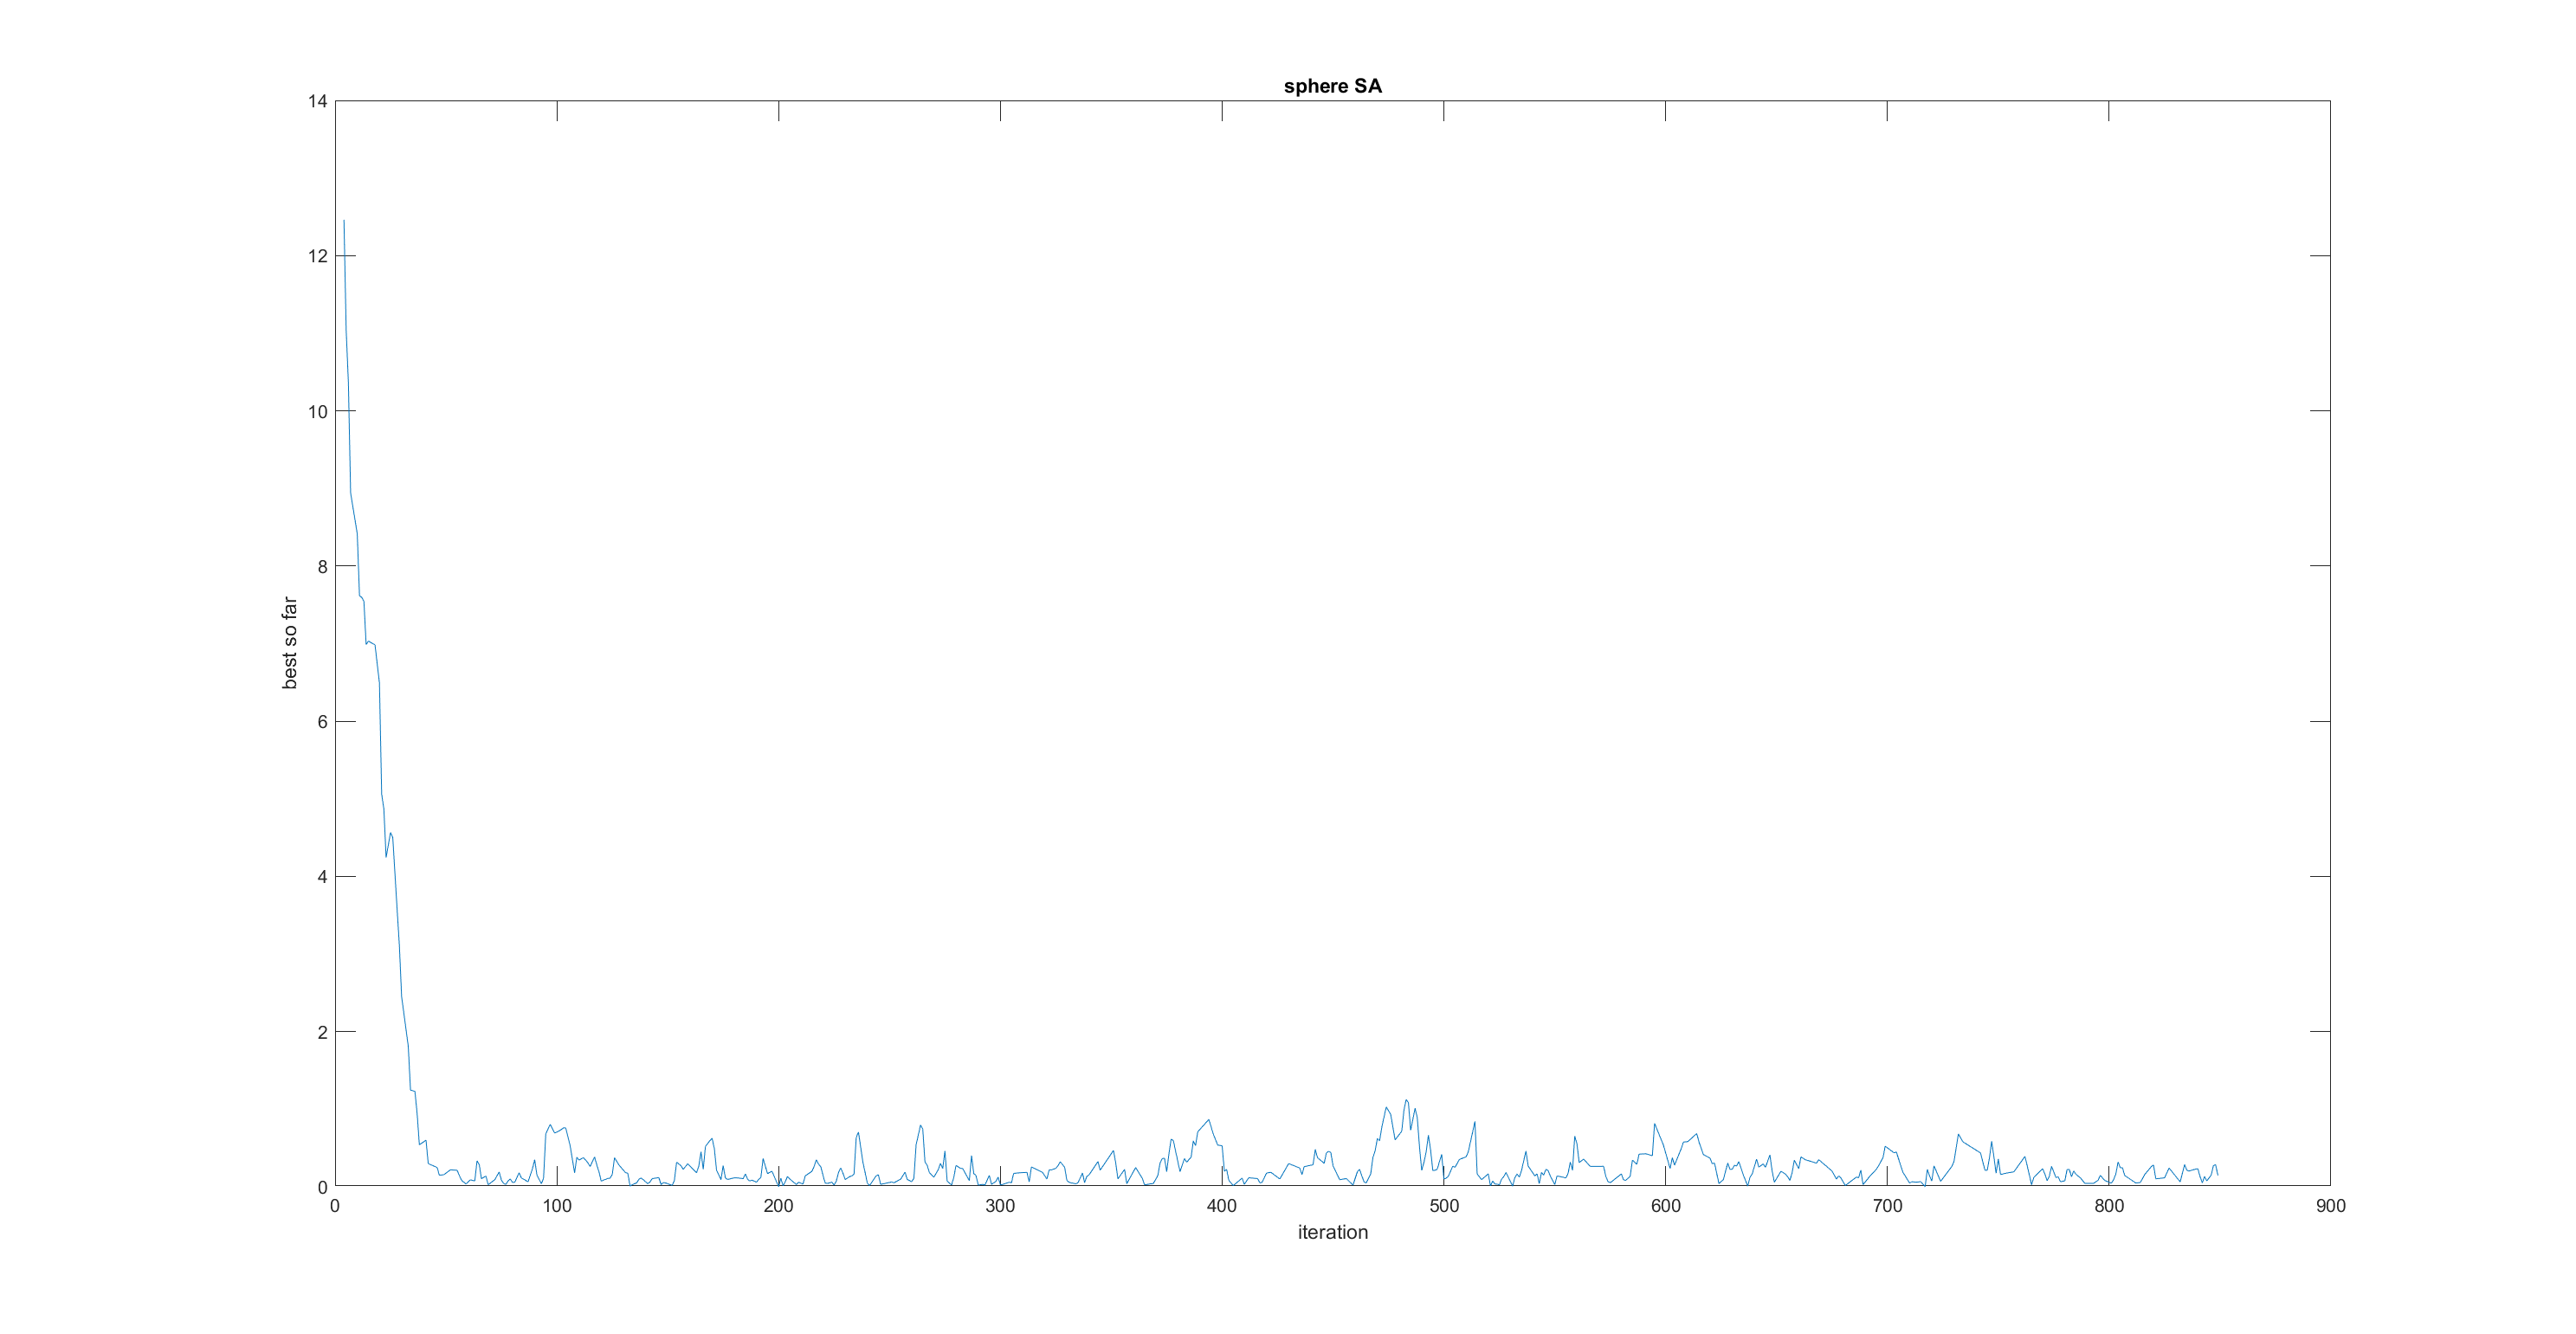
\includegraphics[width=0.45\textwidth]{Q1/figures/sphere_SA.png}
                \caption{Performance of SA on the sphere function}
                \label{fig:sphere_SA}
            \end{figure}

            \begin{figure}[!htbp]
                \centering
                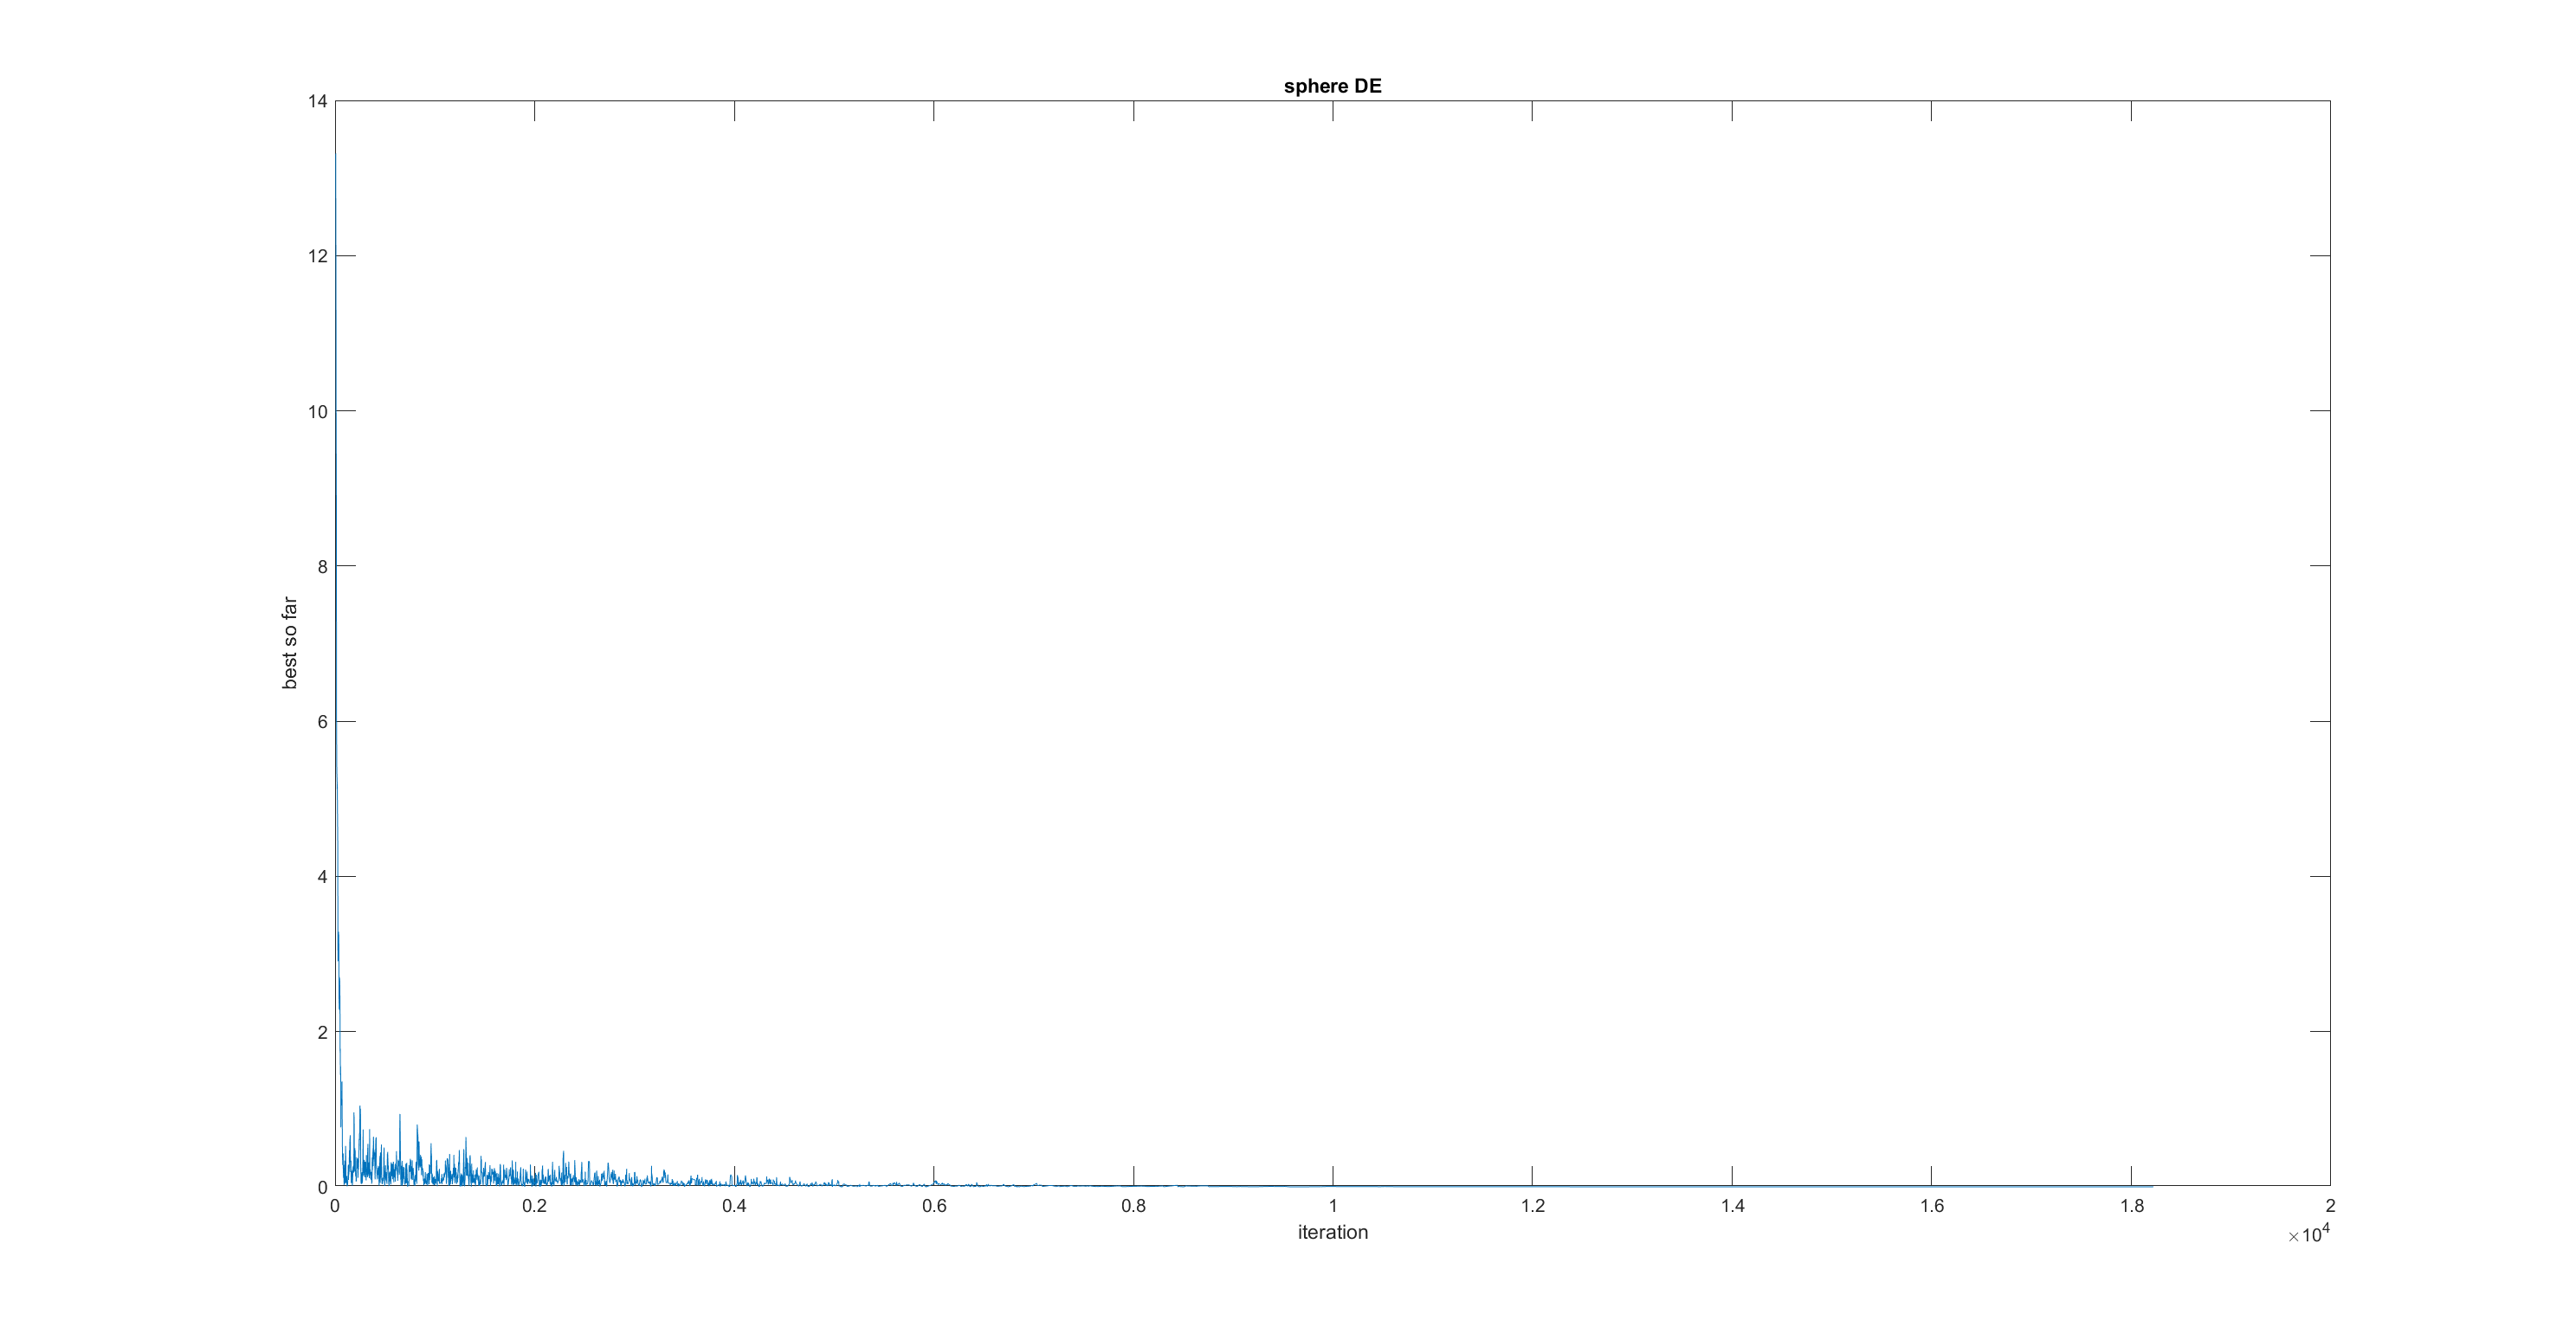
\includegraphics[width=0.45\textwidth]{Q1/figures/sphere_DE.png}
                \caption{Performance of DE on the sphere function}
                \label{fig:sphere_DE}
            \end{figure}
        }

        \subsubsection{The eggholder function}
        {
            Repeated for 20 times, the performance (best value searched and time cost) of each algorithm is recorded. 
            (Table \ref{tab:performance_Q1} and \ref{tab:timecost_Q1})
            (Figure \ref{fig:eggholder_SA} and \ref{fig:eggholder_DE})

            \begin{table}[!hbp]
                \centering
                \begin{tabular}{|c|c|c|c|}
                    \hline
                    Alg. & best so far (min) & b.s.f. (mean) & b.s.f. (max) \\
                    \hline
                    SA &  -959.6406 &  -872.9803 &  -555.5534 \\
                    \hline
                    DE &  -959.6407 &  -959.6404 &  -959.6386 \\
                    \hline
                \end{tabular}
                \caption{Performance after 20th repitition}
                \label{tab:performance_Q1}
            \end{table}

            \begin{table}[!hbp]
                \centering
                \begin{tabular}{|c|c|c|c|}
                    \hline
                    Alg. & time cost in sec (min) & t.c. (mean) & t.c. (max) \\
                    \hline
                    SA &  0 &  0.0055 &  0.0469 \\
                    \hline
                    DE &  5.2656 &  6.6070 &  8.9688 \\
                    \hline
                \end{tabular}
                \caption{Time cost after 20th repitition}
                \label{tab:timecost_Q1}
            \end{table}

            \begin{figure}[!htbp]
                \centering
                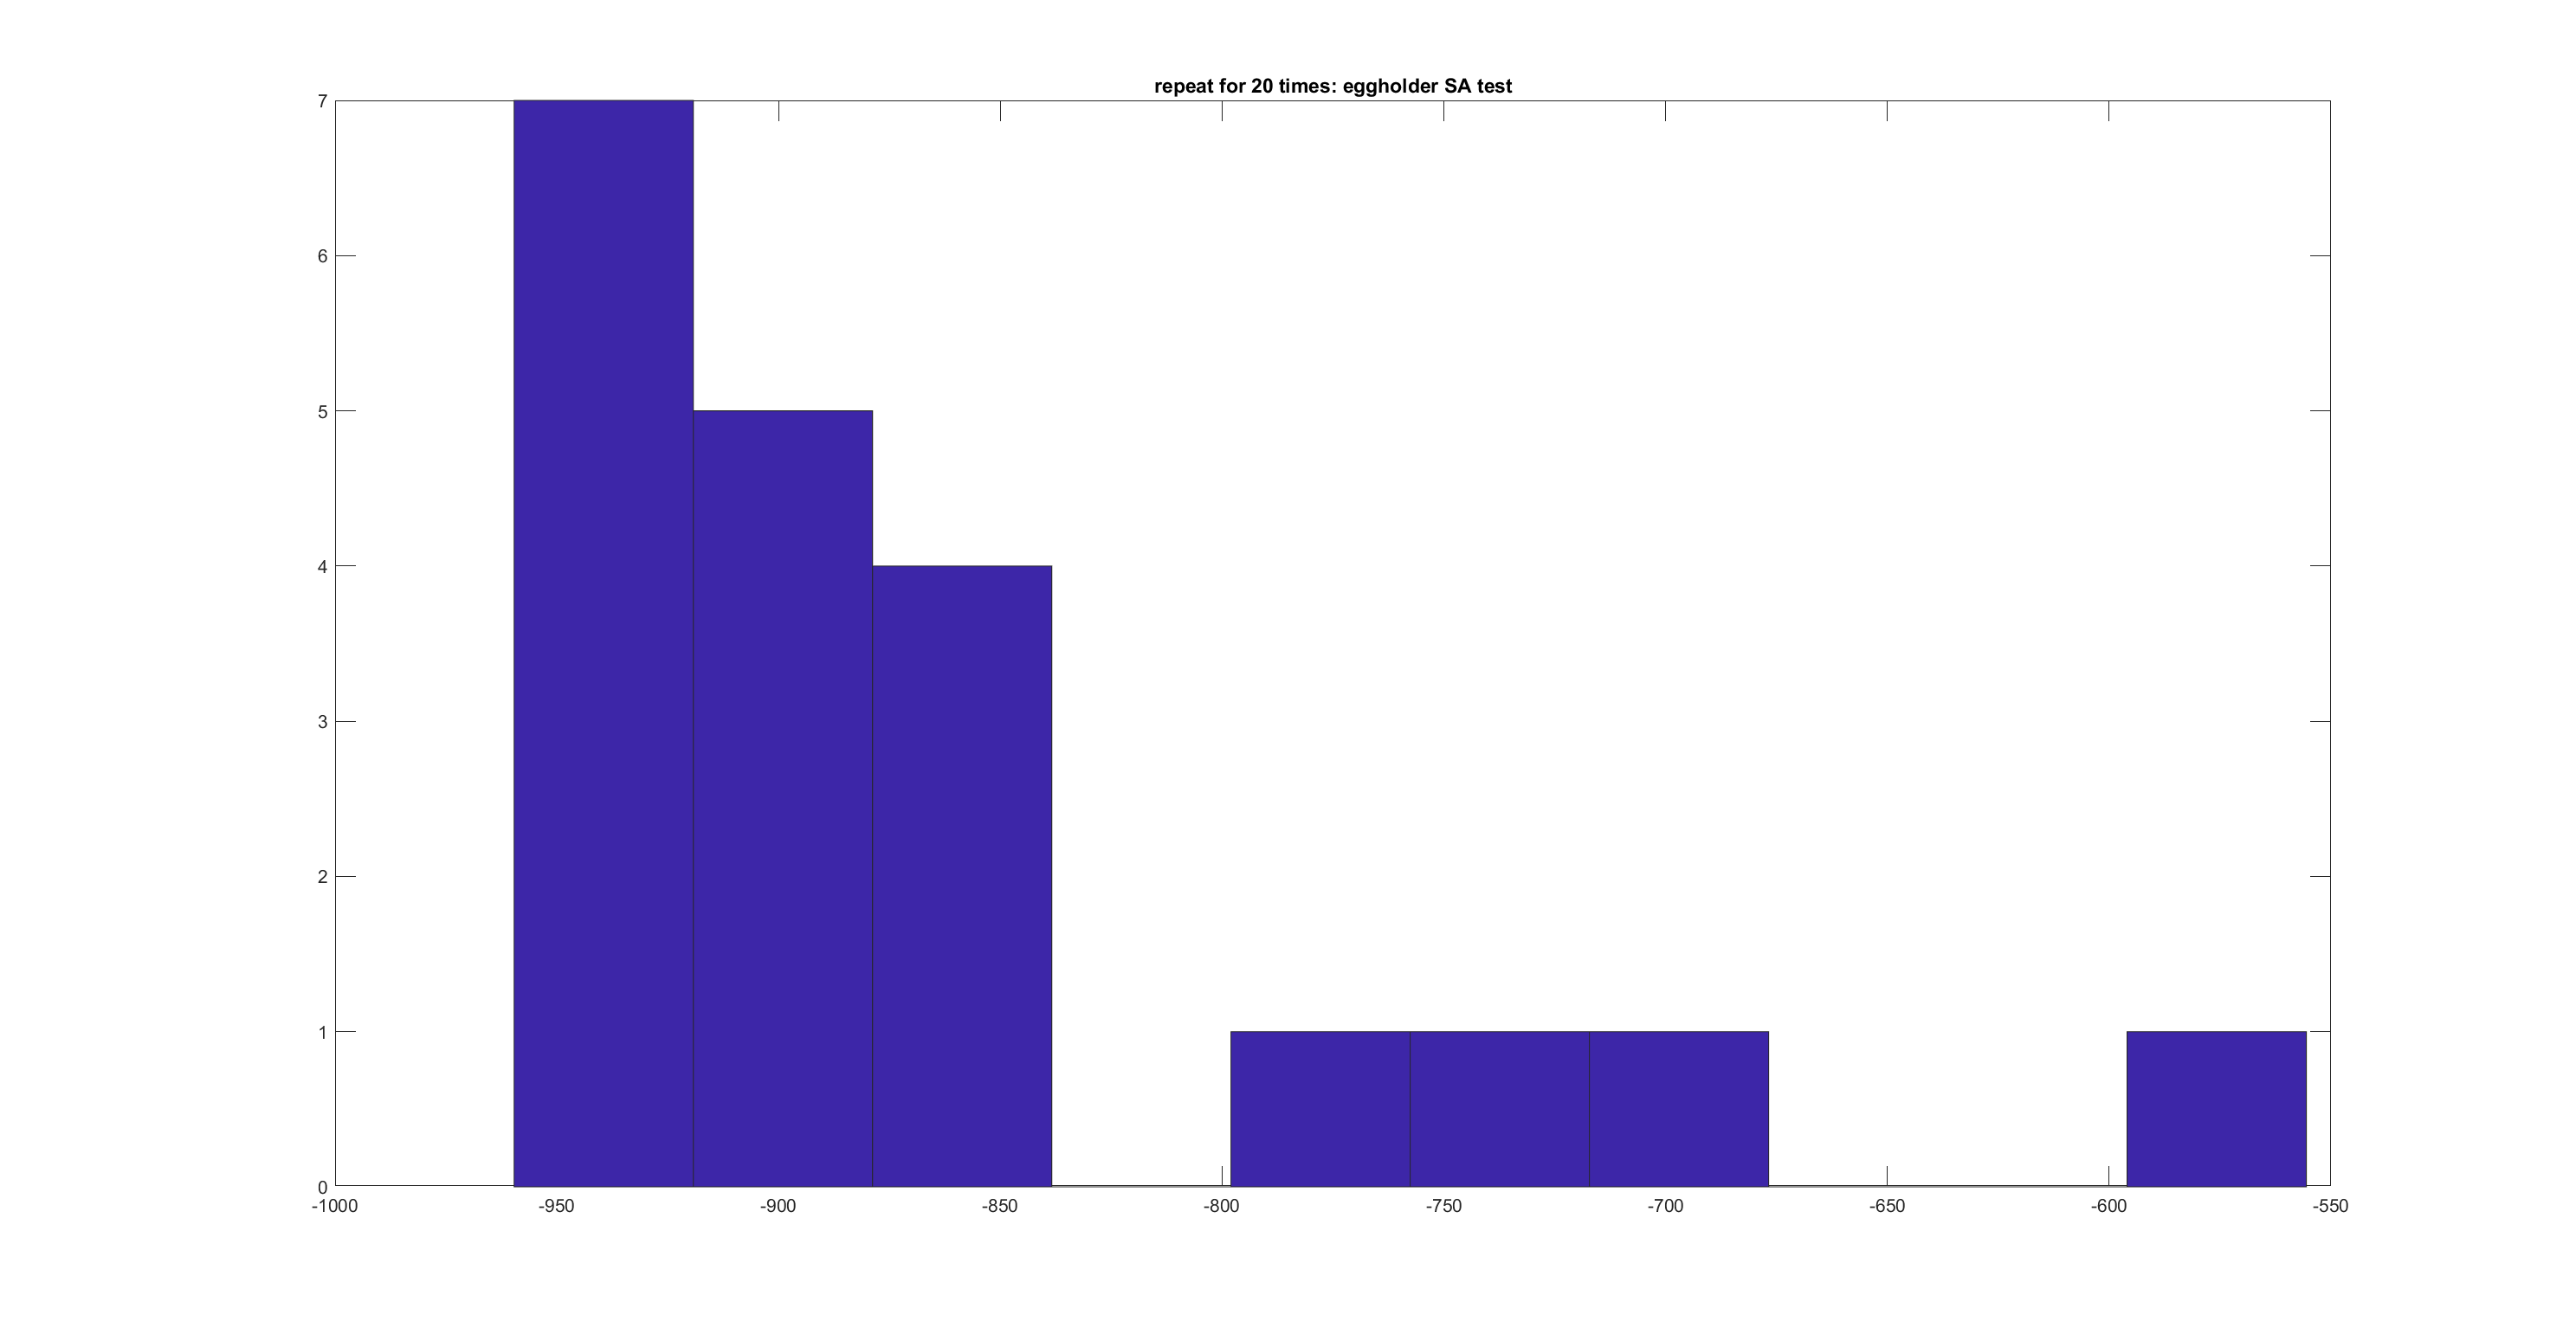
\includegraphics[width=0.45\textwidth]{Q1/figures/eggholder_SA_test.png}
                \caption{Performance of SA after 20th repitition}
                \label{fig:eggholder_SA}
            \end{figure}

            \begin{figure}[!htbp]
                \centering
                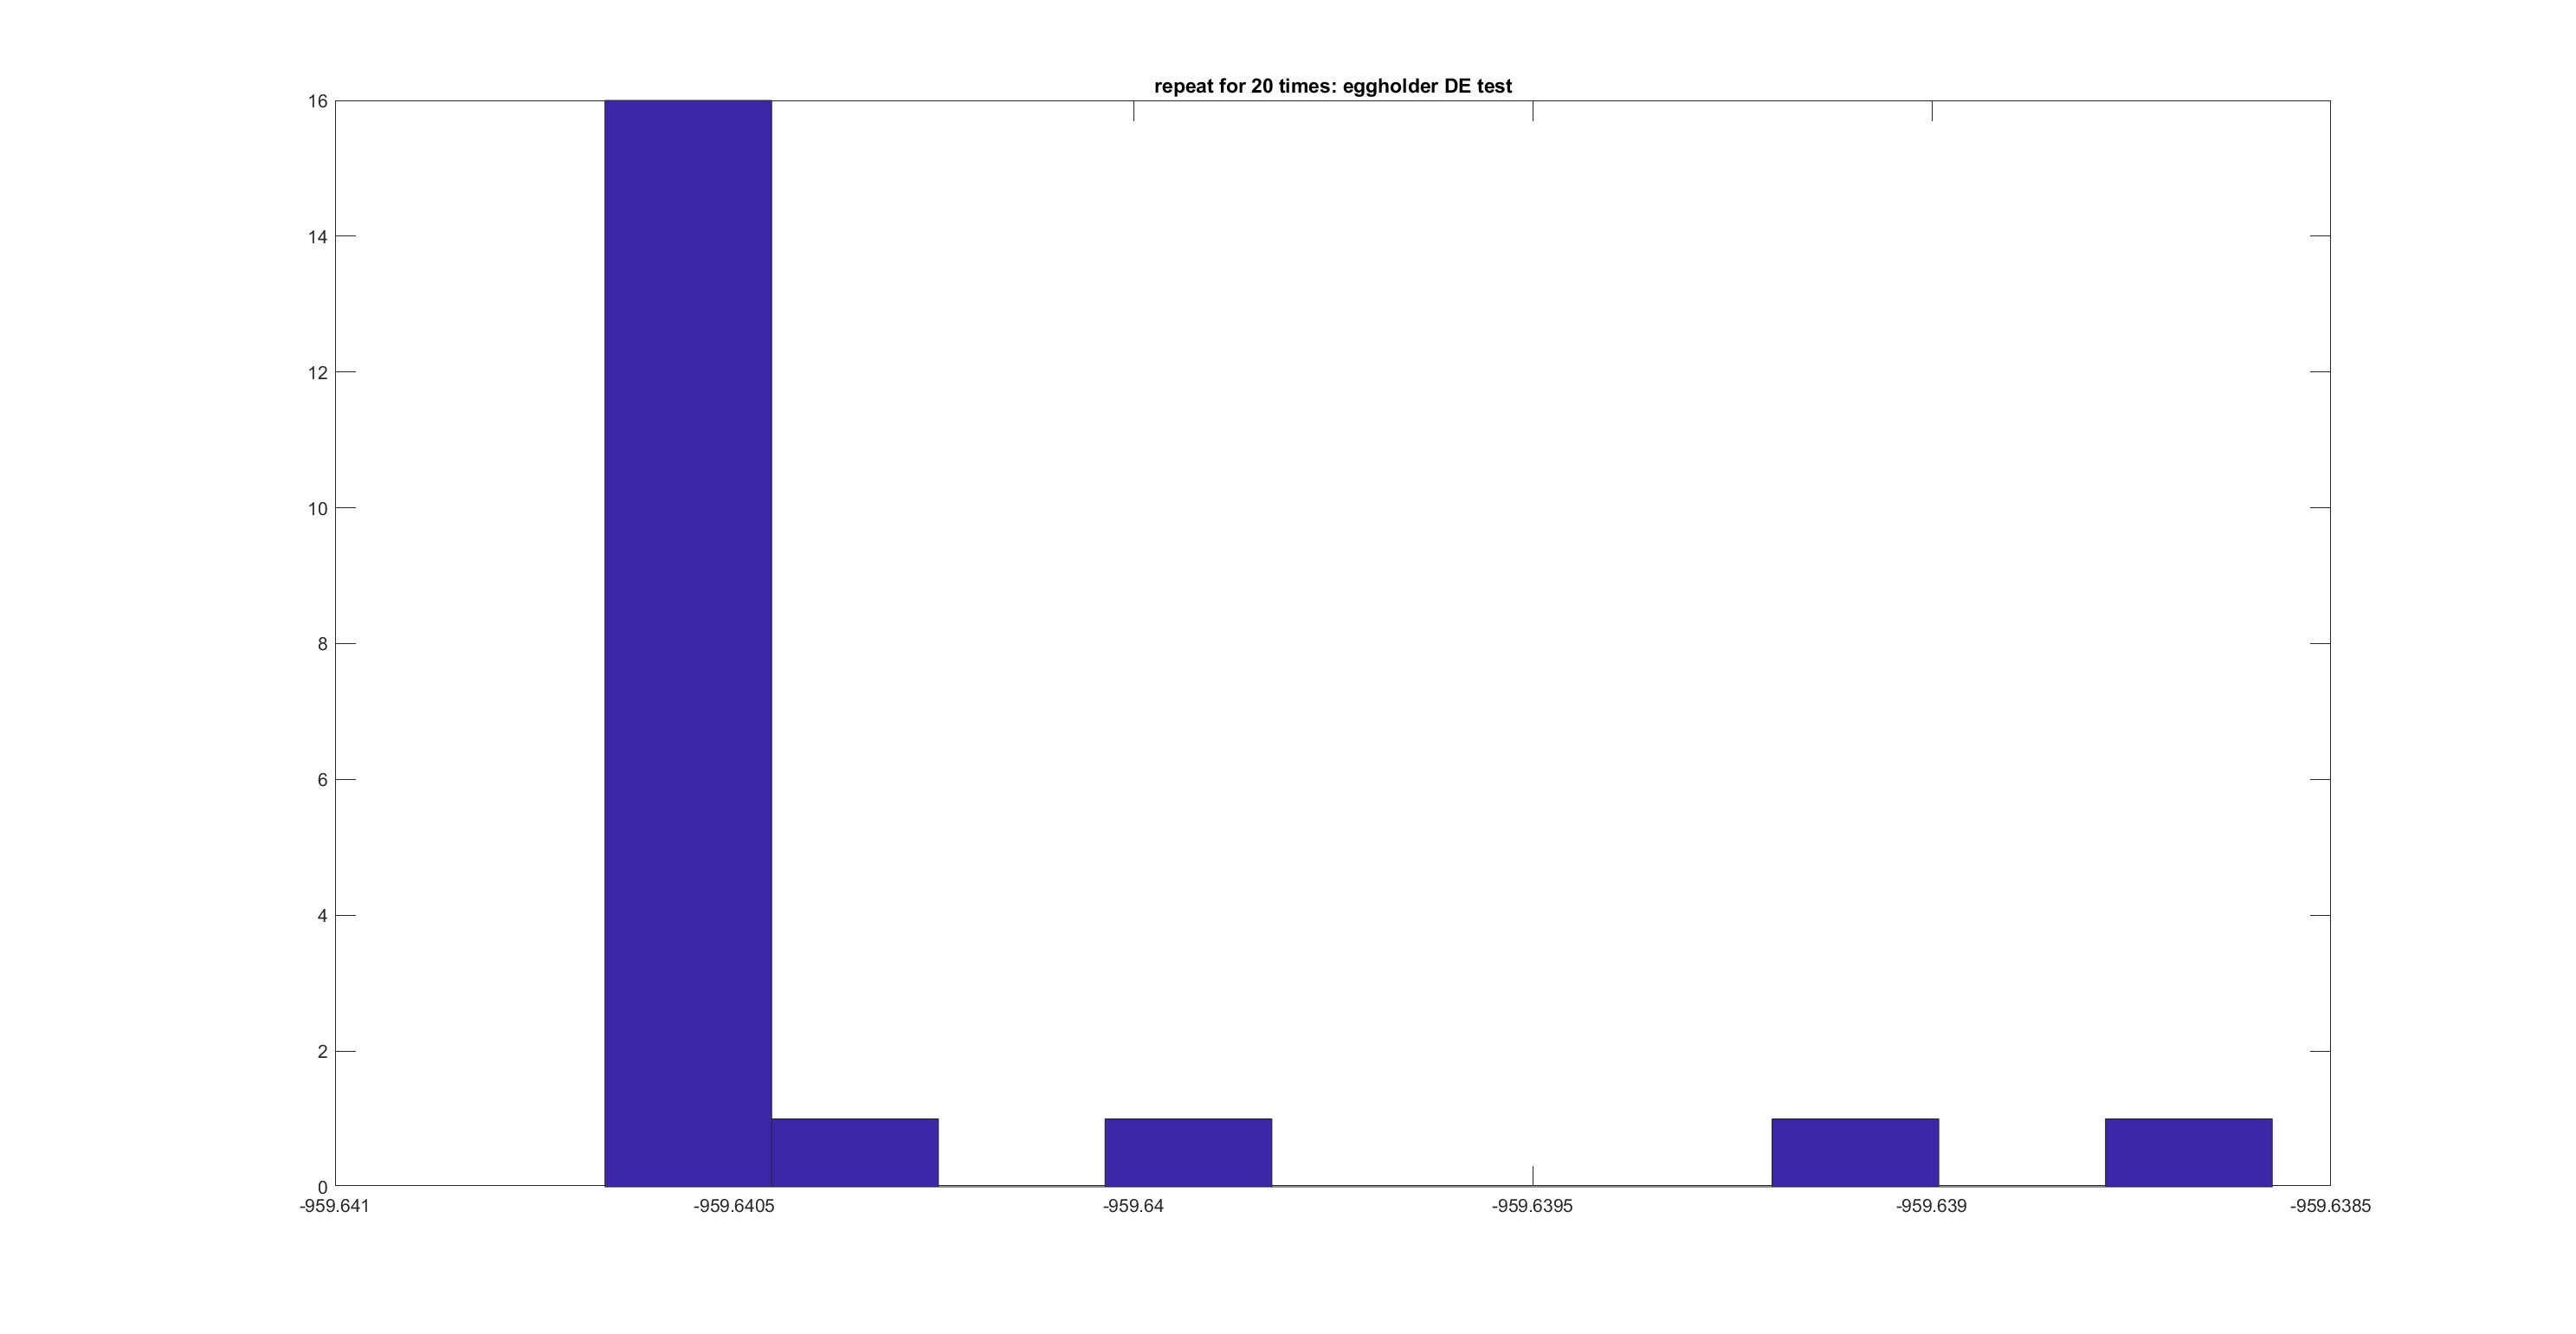
\includegraphics[width=0.45\textwidth]{Q1/figures/eggholder_DE_test.png}
                \caption{Performance of DE after 20th repitition}
                \label{fig:eggholder_DE}
            \end{figure}

            \begin{itemize}
                \item Performance: DE wins. DE always manages to find the global minimum at -959.64, while SA cannot. 
                Although SA did find the global minimum occasionally, the average performance is -872, which is still far from the best value.
                \item Time cost: SA wins. SA has little time cost, consuming 47 milliseconds in the worst case. 
                In contrast, it always takes seconds for DE to complete, because it is population-based rather than individual-based. 
                Obviously, the time cost of DE is proportional to the population size. 
                With a small population size, DE has a time cost affordable in certain circumstances.
            \end{itemize}
        }

        \subsubsection{Plots of best-so-fars}
        {
            \begin{figure}[!htbp]
                \centering
                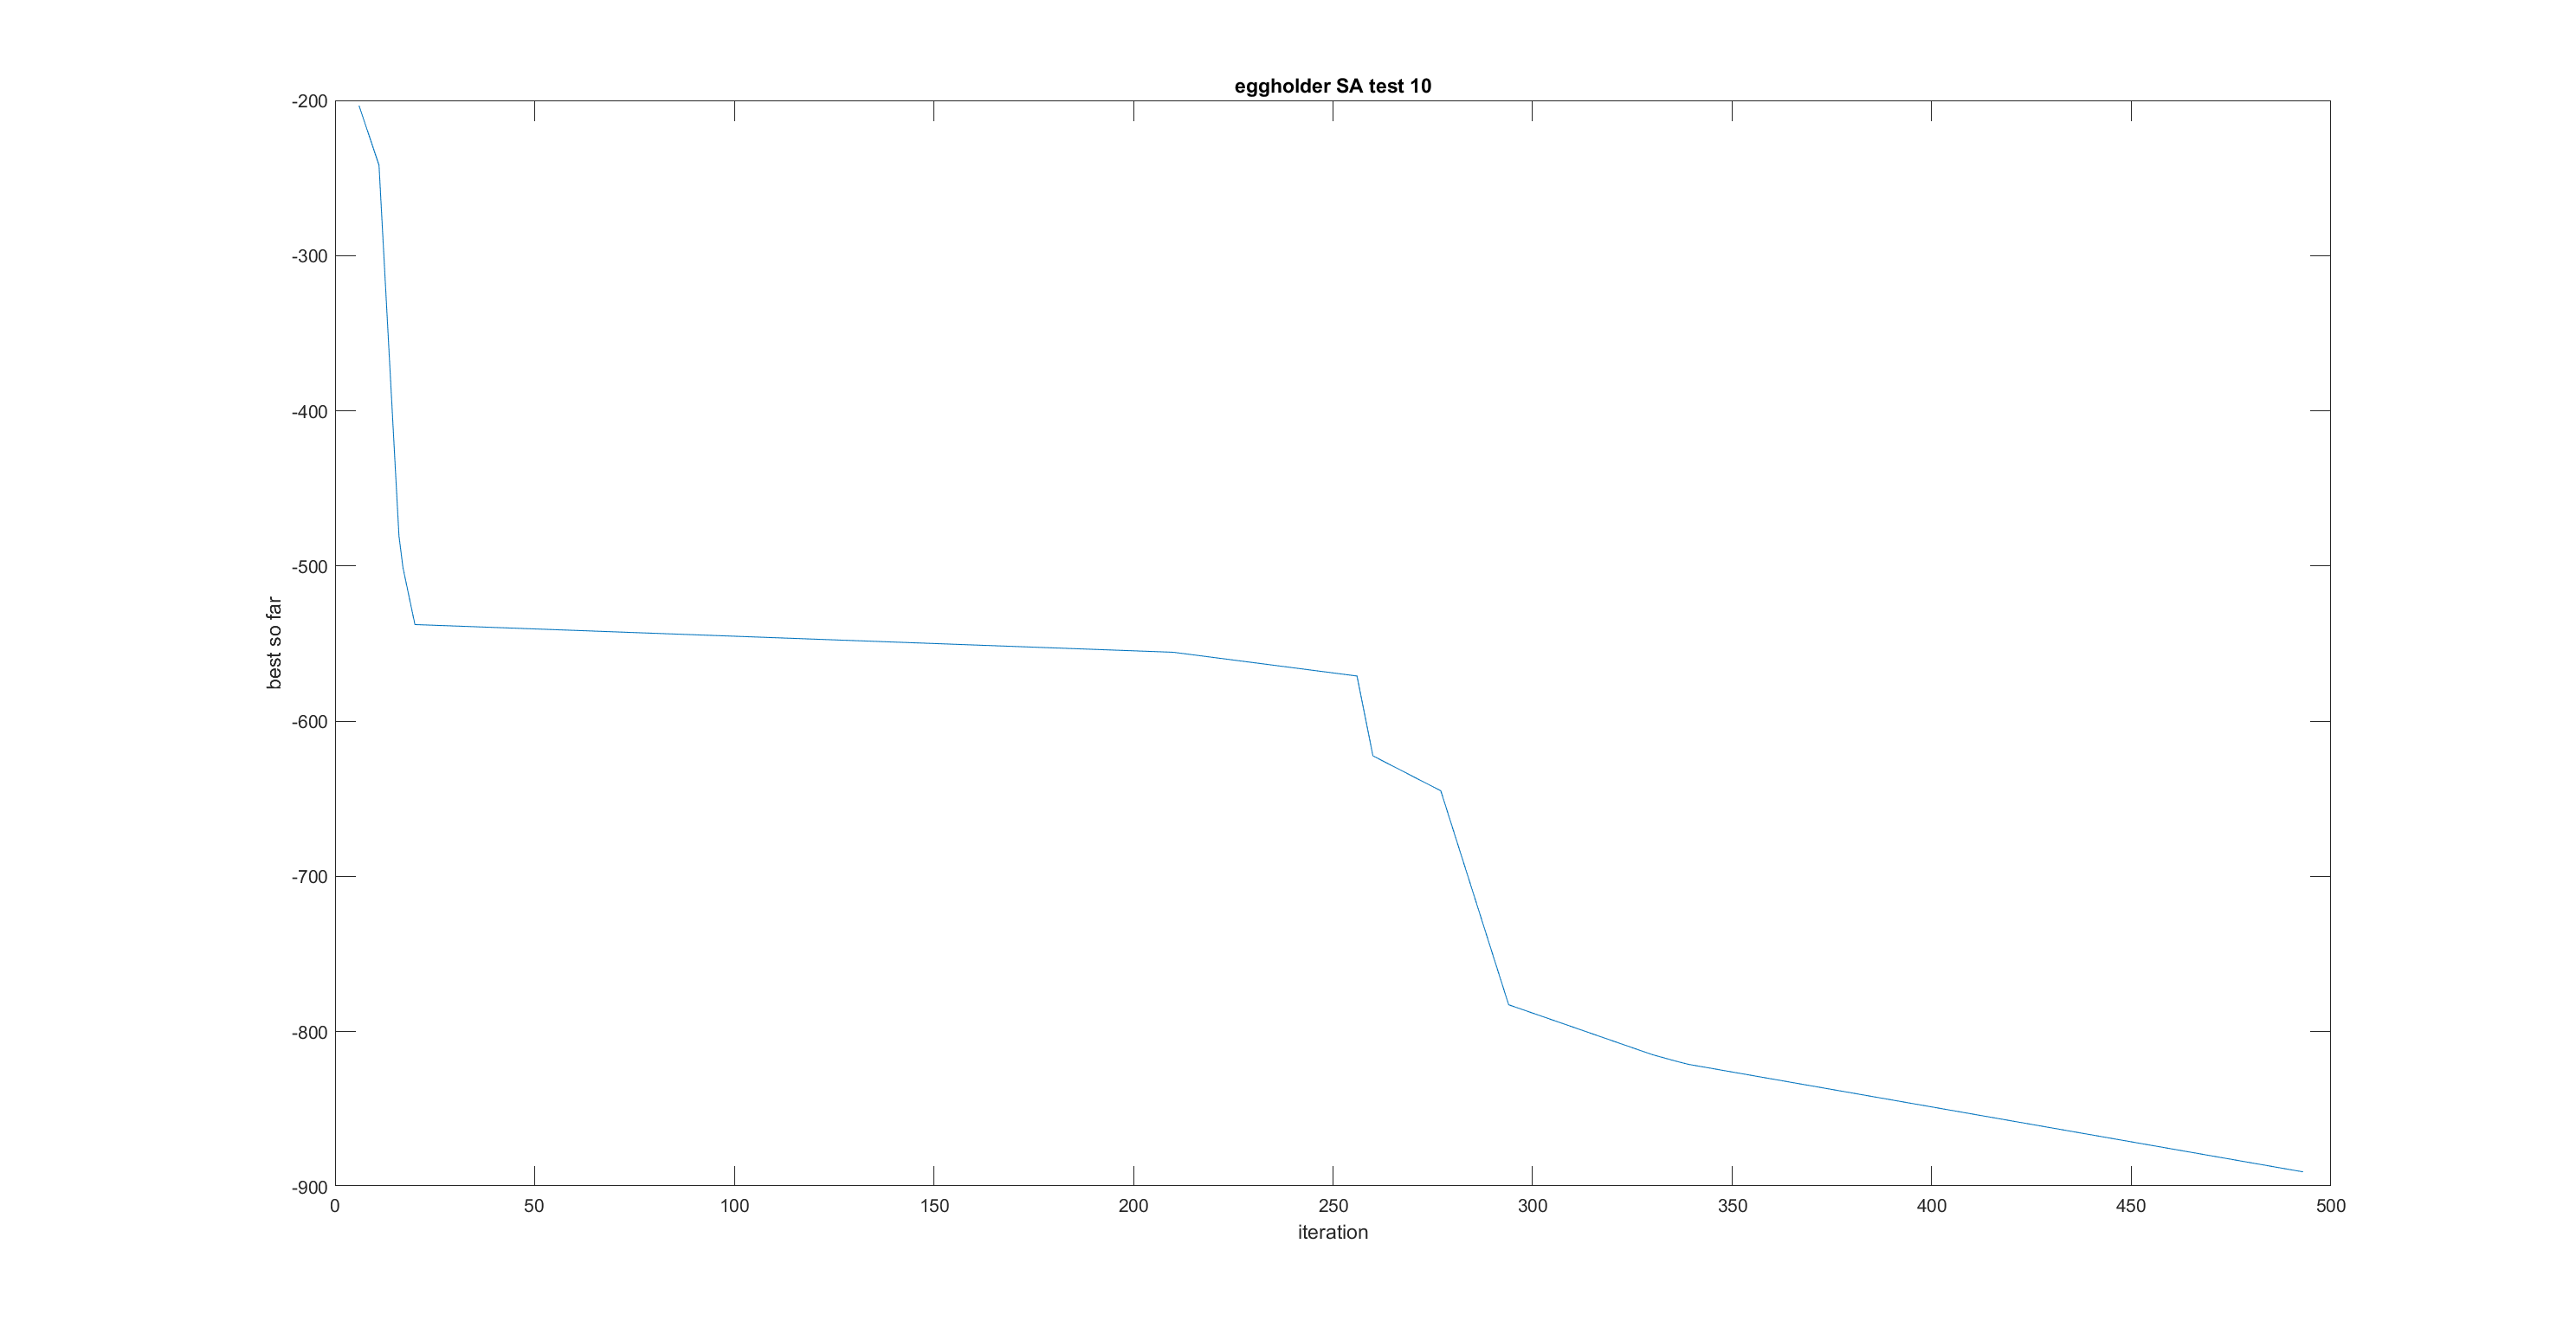
\includegraphics[width=0.45\textwidth]{Q1/figures/eggholder_SA_test_10.png}
                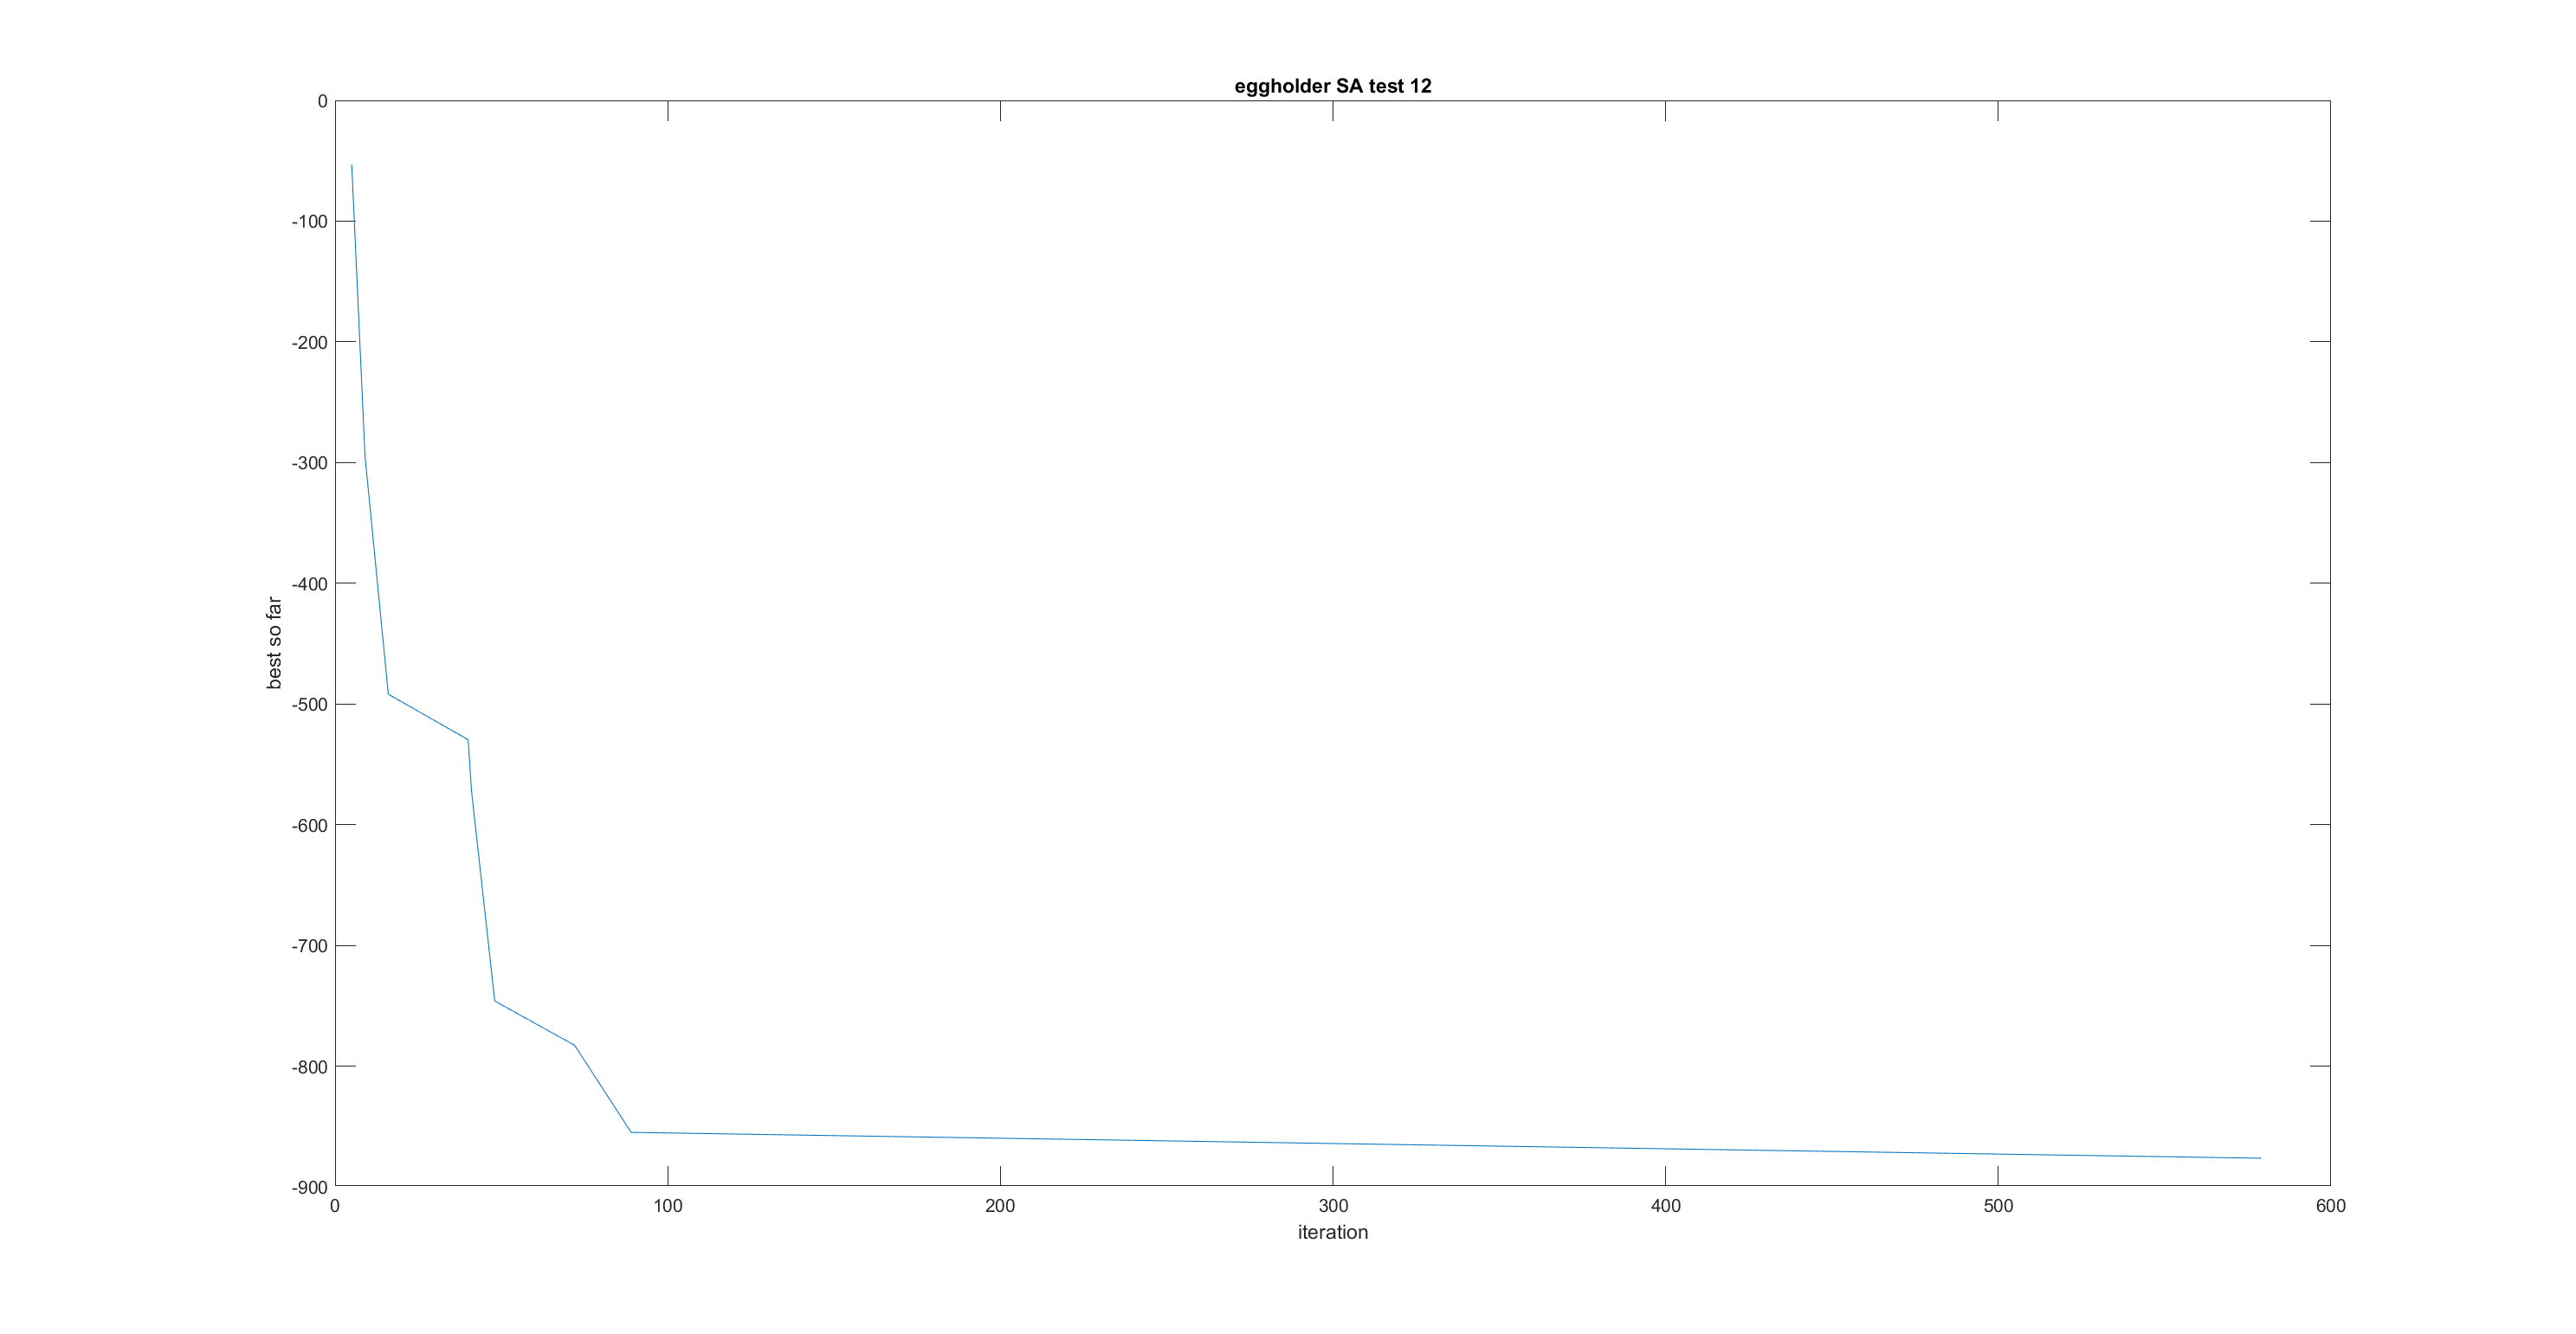
\includegraphics[width=0.45\textwidth]{Q1/figures/eggholder_SA_test_12.png}
                \caption{10th and 12th test of SA}
                \label{fig:plots_SA}
            \end{figure}

            \begin{figure}[!htbp]
                \centering
                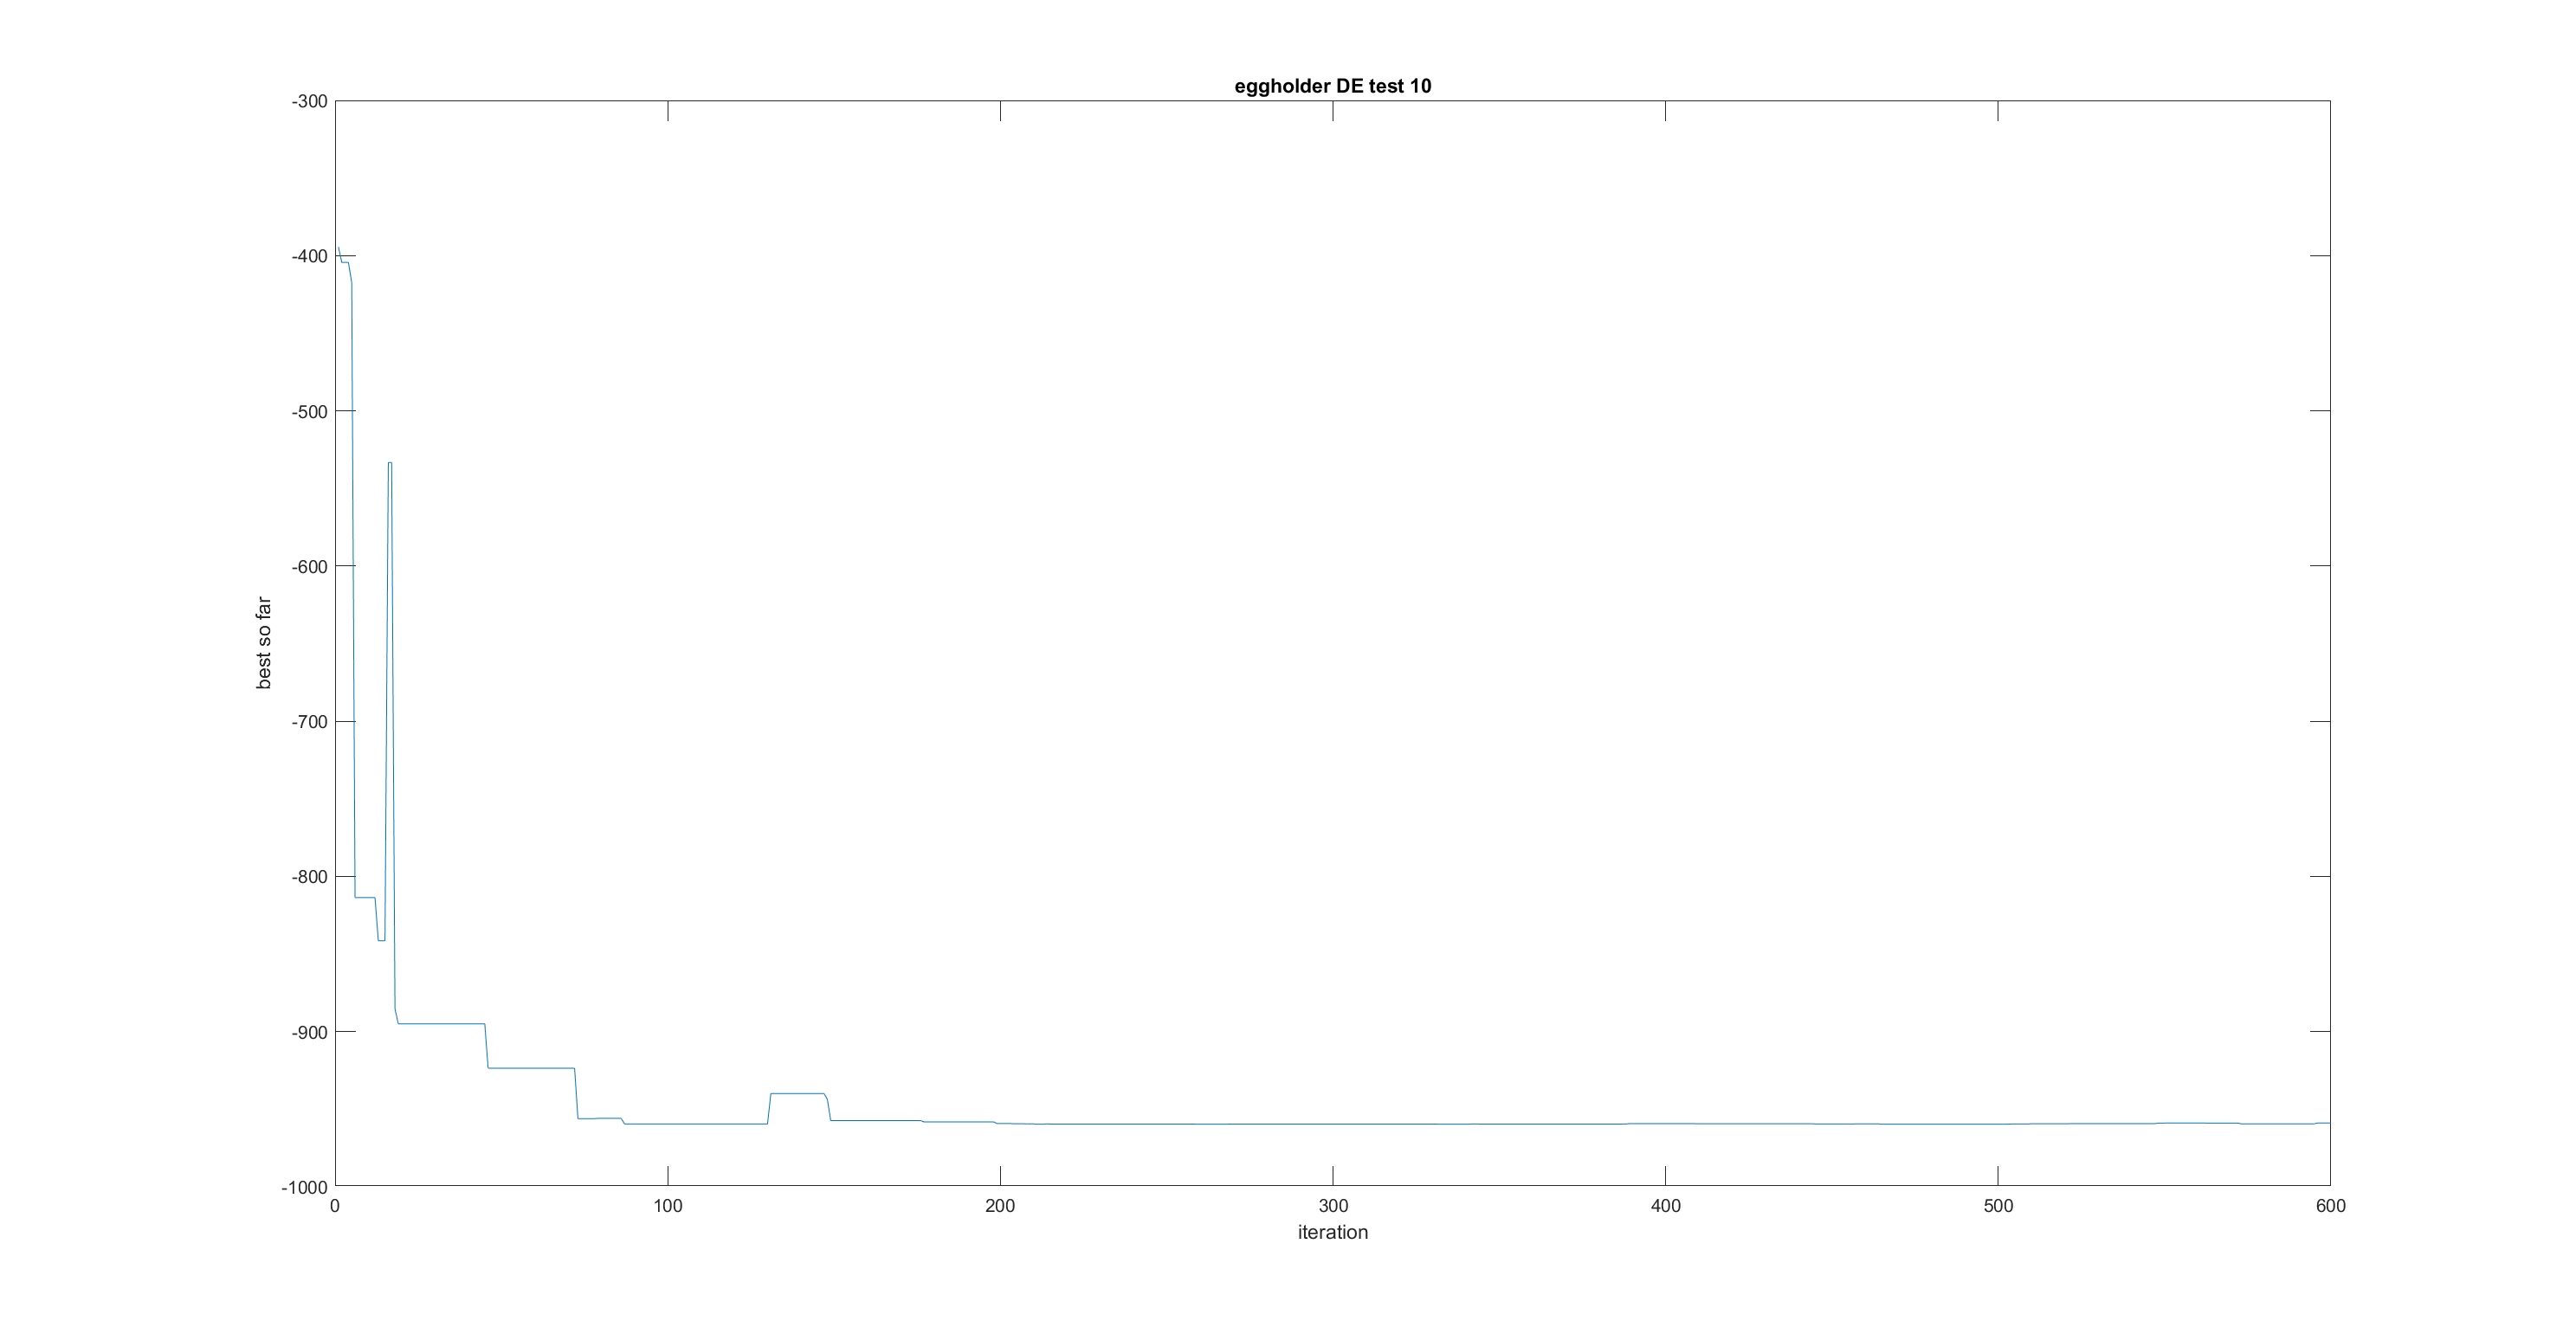
\includegraphics[width=0.45\textwidth]{Q1/figures/eggholder_DE_test_10.png}
                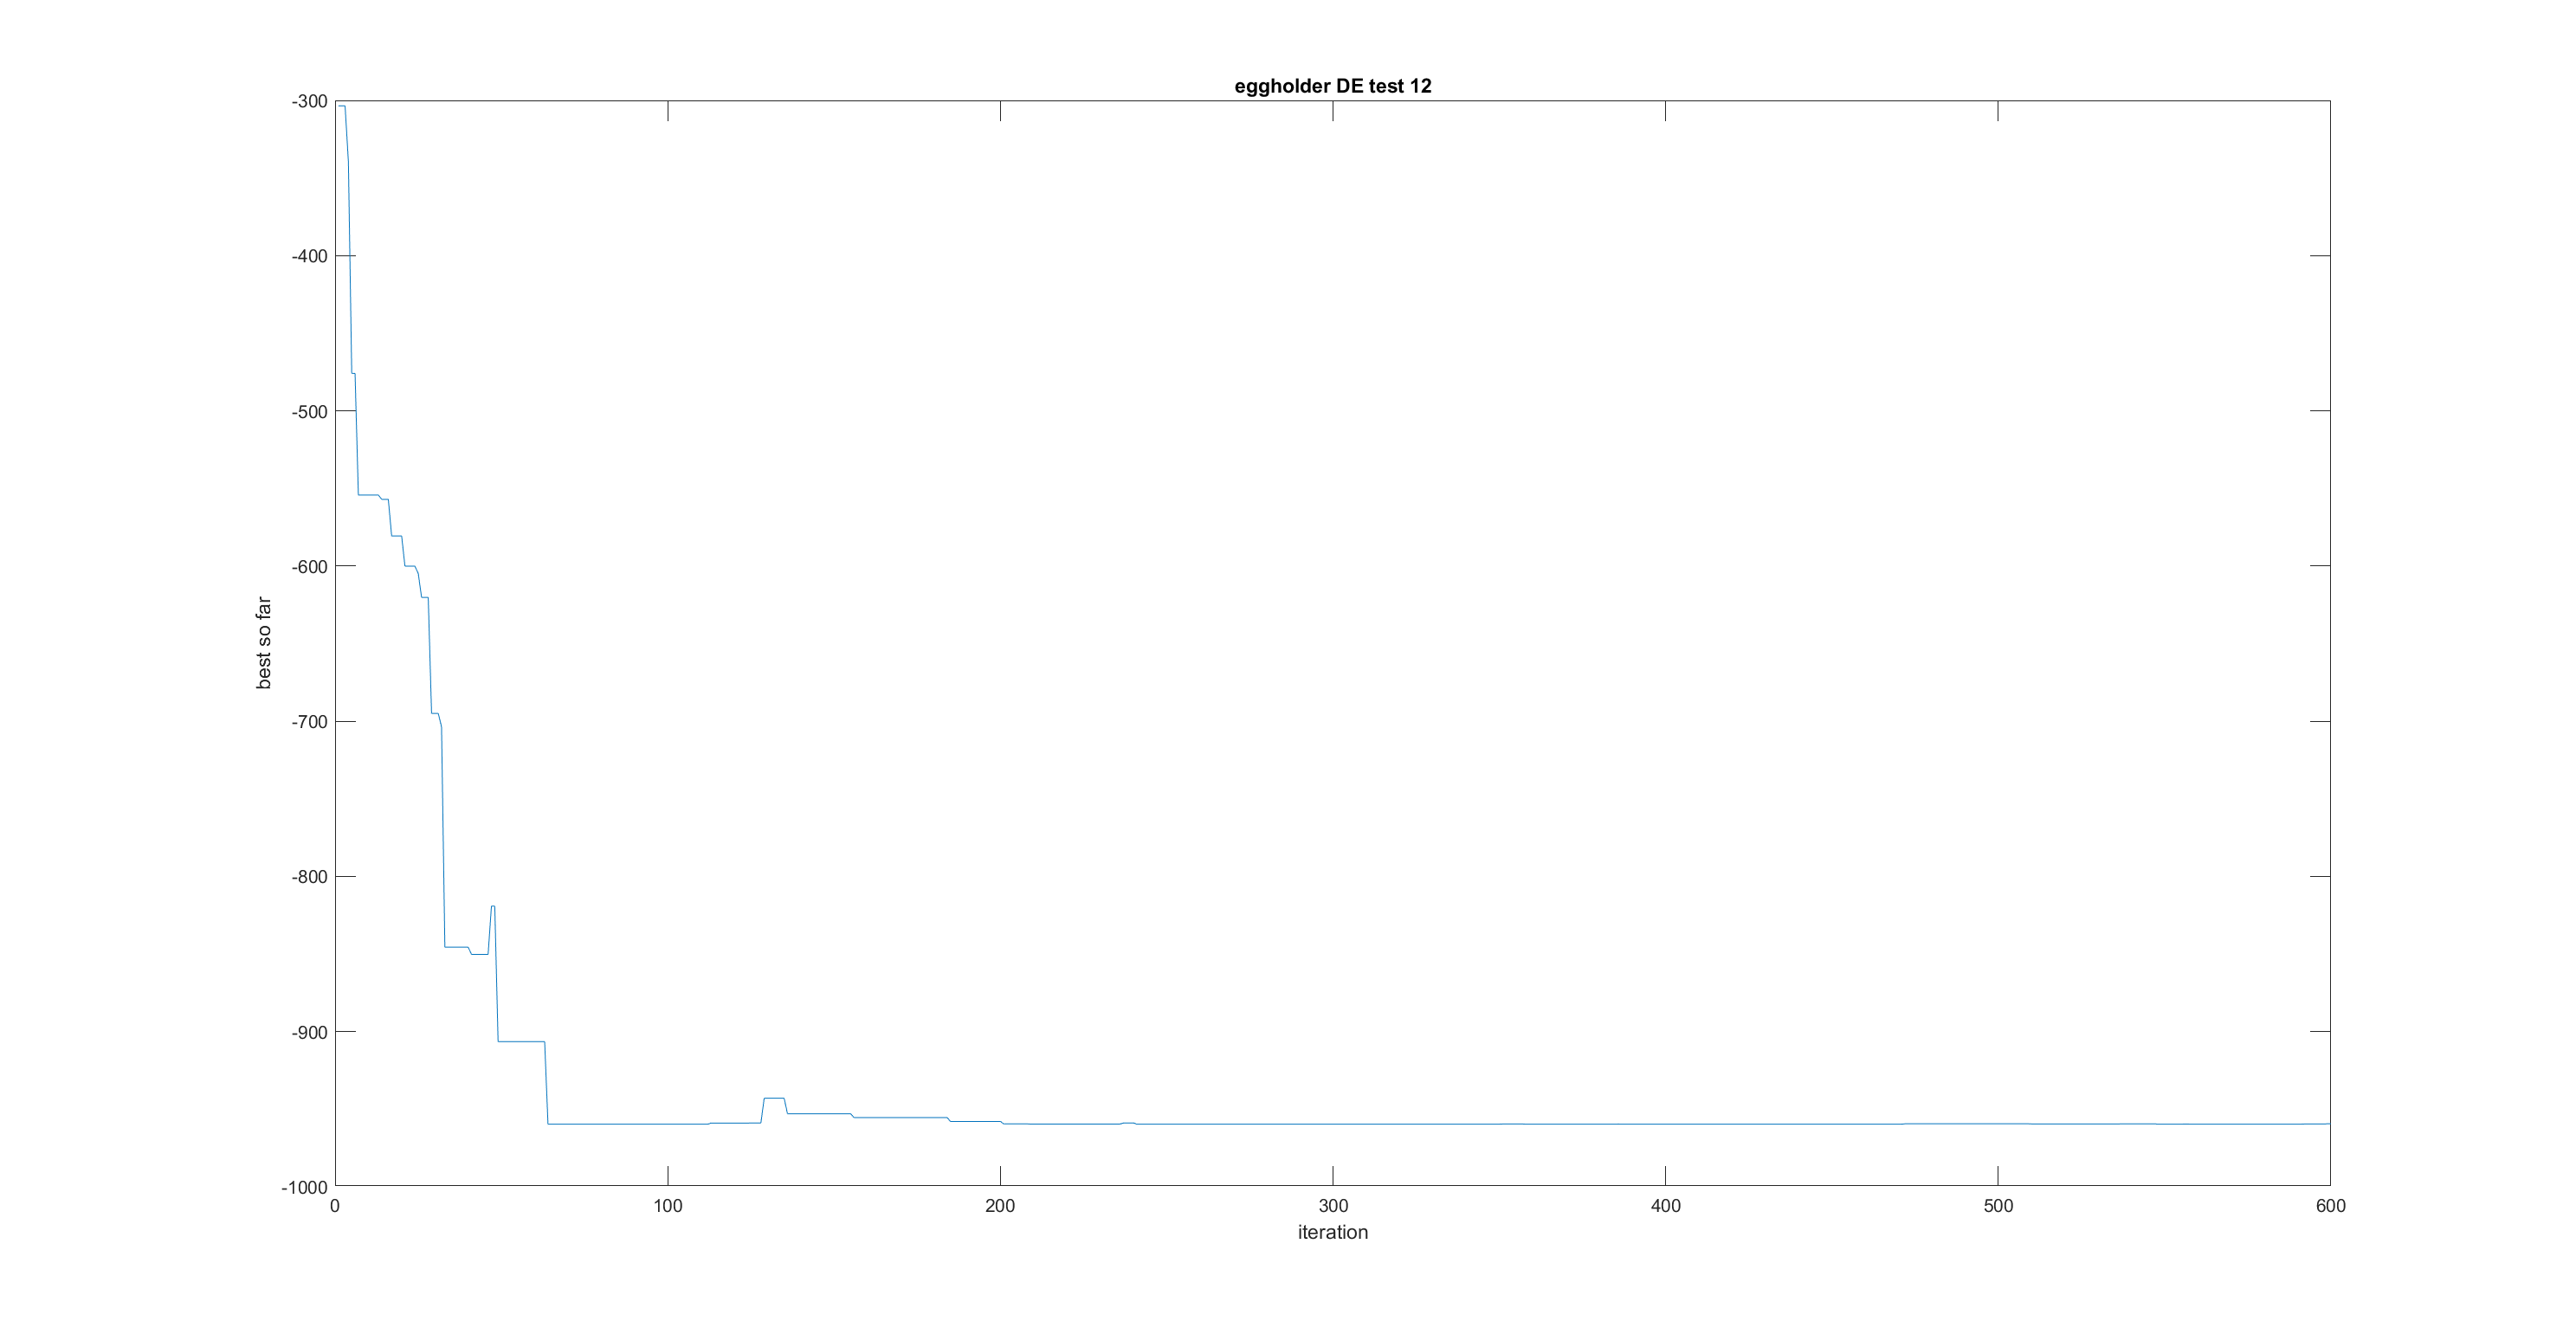
\includegraphics[width=0.45\textwidth]{Q1/figures/eggholder_DE_test_12.png}
                \caption{10th and 12th test of DE}
                \label{fig:plots_DE}
            \end{figure}

            From Figure \ref{fig:plots_SA} and \ref{fig:plots_DE}, we see that
            \begin{itemize}
                \item The number of iterations needed for SA varies a lot. For test 10, it took 400 epochs. For test 12, only 200 is enough.
                \item DE is much more stationary. Although it is not a monotonic descent, it converges very quickly.
            \end{itemize}
        }
    }

    \subsection{Sensitivity Analysis}
    {
        Hyper tuning could be one of the most tricky parts in an intelligent optimization algorithm. 
        For the tests above, the following hyperparameters are used. (Table \ref{tab:hyper_SA_Q1} and \ref{tab:hyper_DE_Q1})

        \begin{table}[!hbp]
            \centering
            \begin{tabular}{|c|c|}
                \hline
                Hyperparameter & Default value \\
                \hline
                initial temperature & 0.2 \\
                \hline
                annealing rate & 0.98 \\
                \hline
                std. for proposal func. & 100 \\
                \hline
                inner loop iterations & 20 \\
                \hline
                outer loop iterations & 30 \\
                \hline
            \end{tabular}
            \caption{Default Hypers for SA}
            \label{tab:hyper_SA_Q1}
        \end{table}

        \begin{table}[!hbp]
            \centering
            \begin{tabular}{|c|c|}
                \hline
                Hyperparameter & Default value \\
                \hline
                F (mutation) & 0.5 \\
                \hline
                cross rate & 0.3 \\
                \hline
                loop iterations & 600 \\
                \hline
            \end{tabular}
            \caption{Default Hypers for DE}
            \label{tab:hyper_DE_Q1}
        \end{table}

        \begin{figure}[!htbp]
            \centering
            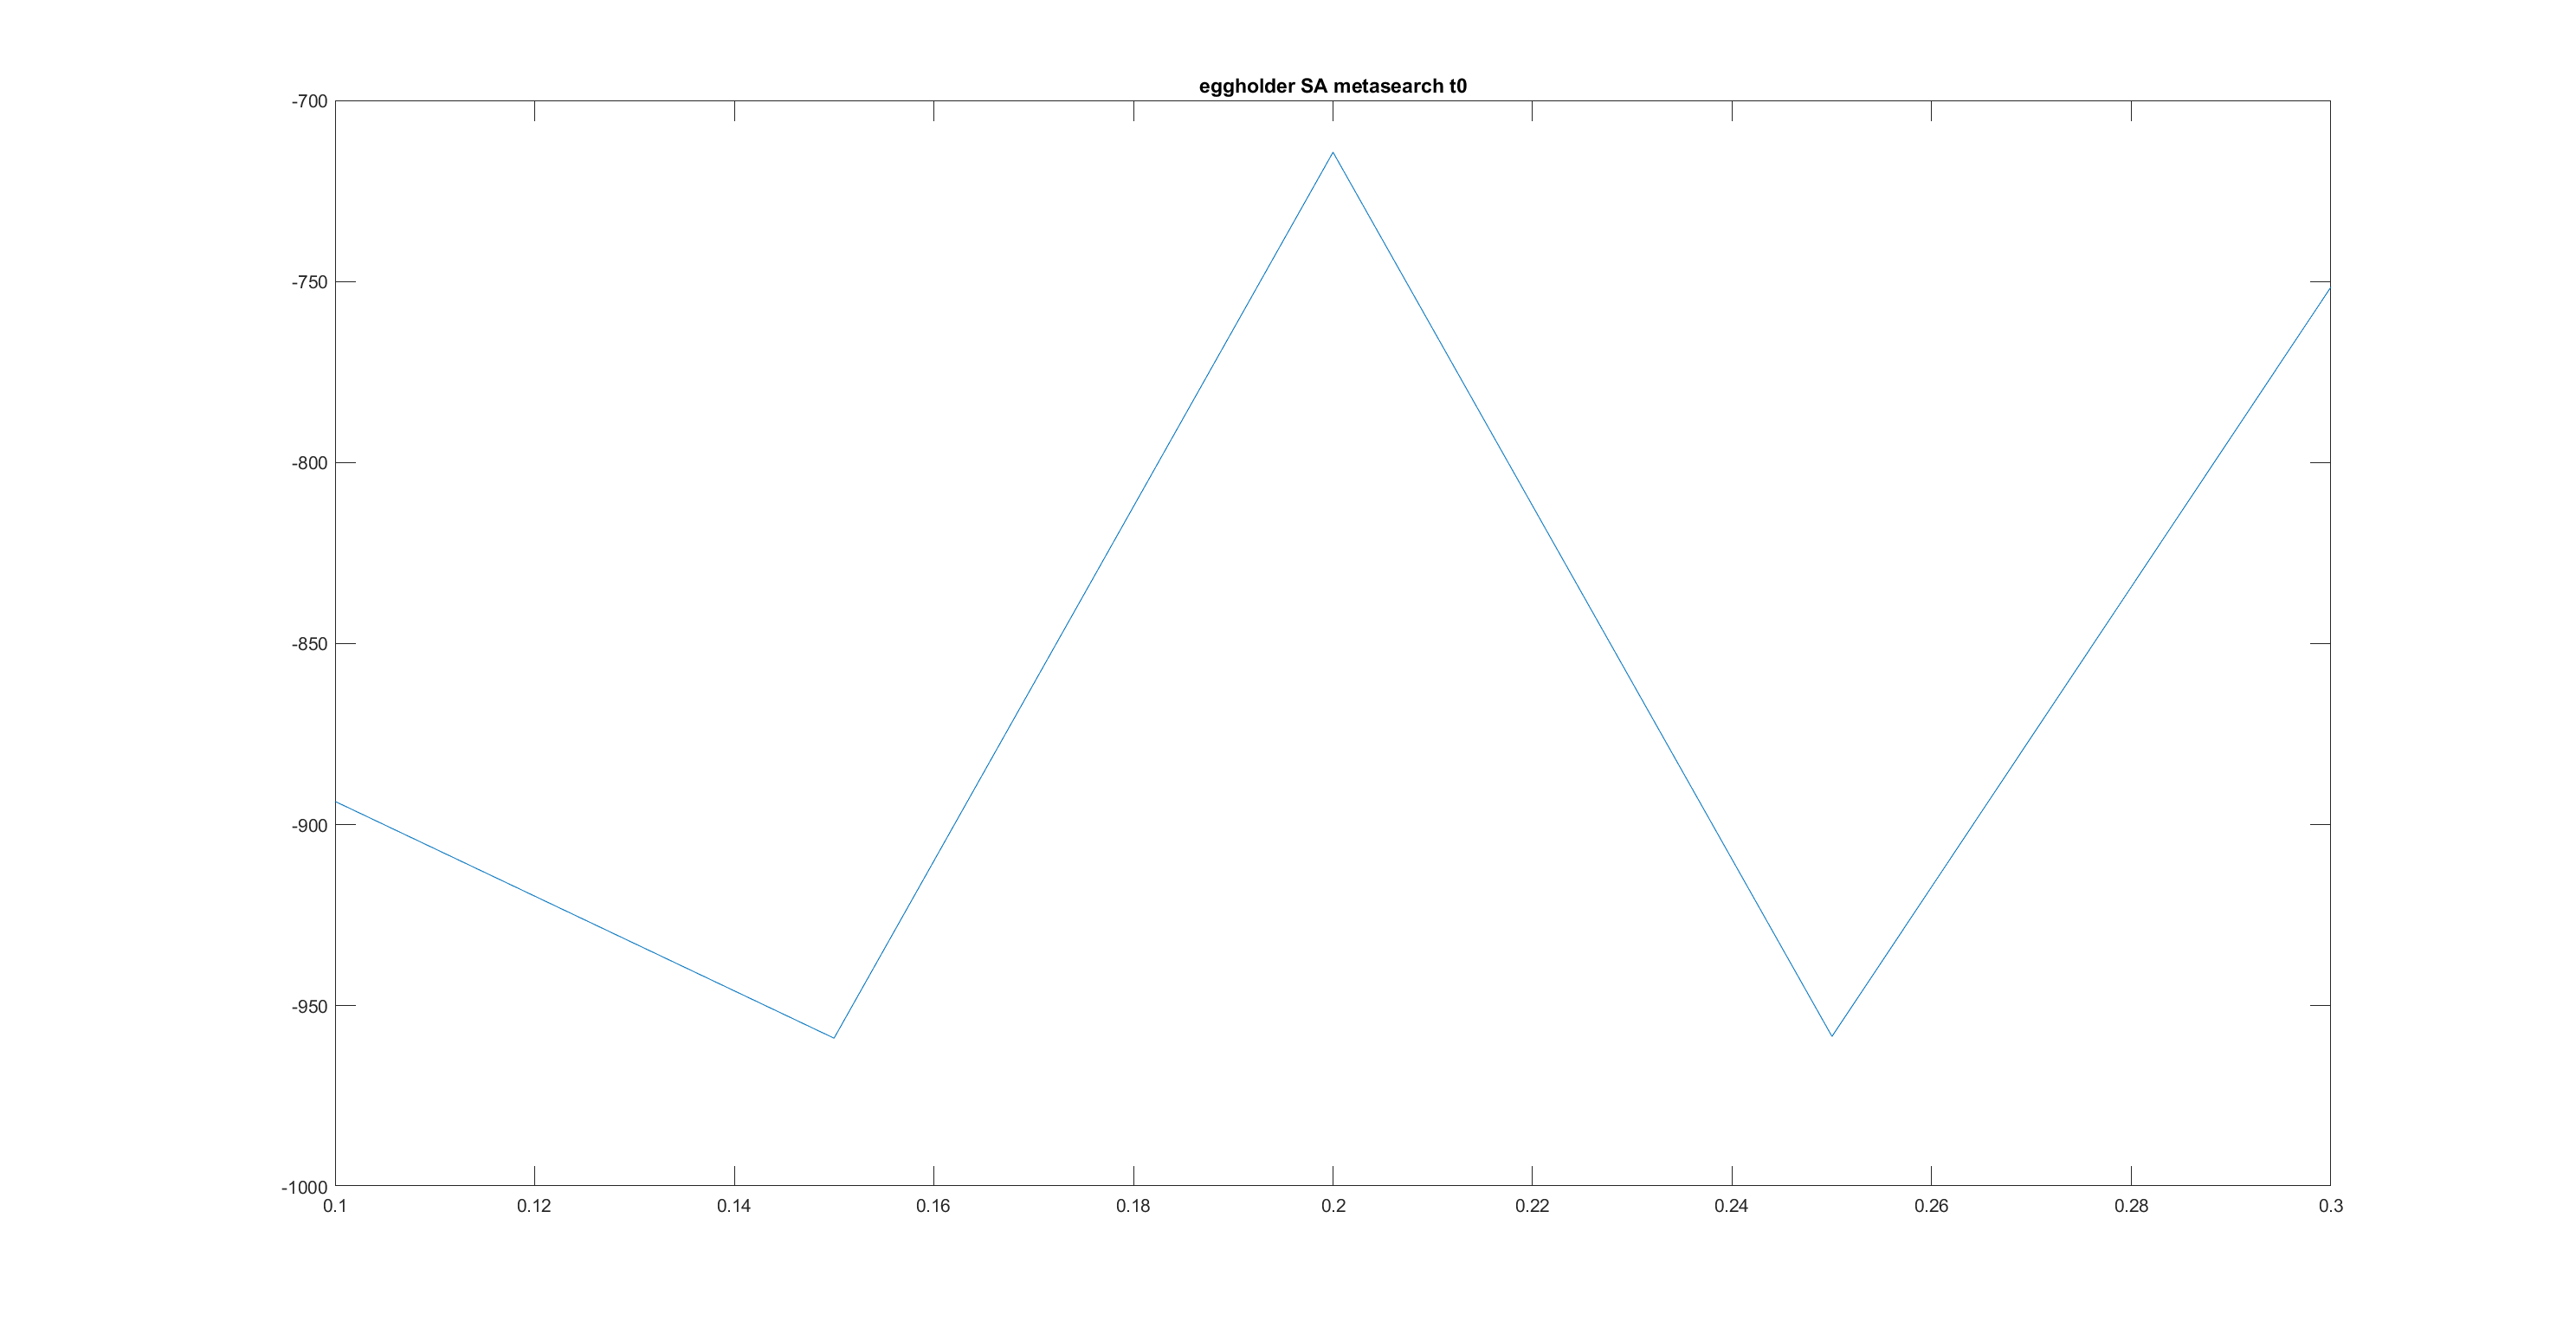
\includegraphics[width=0.45\textwidth]{Q1/figures/eggholder_SA_metasearch_t0.png}
            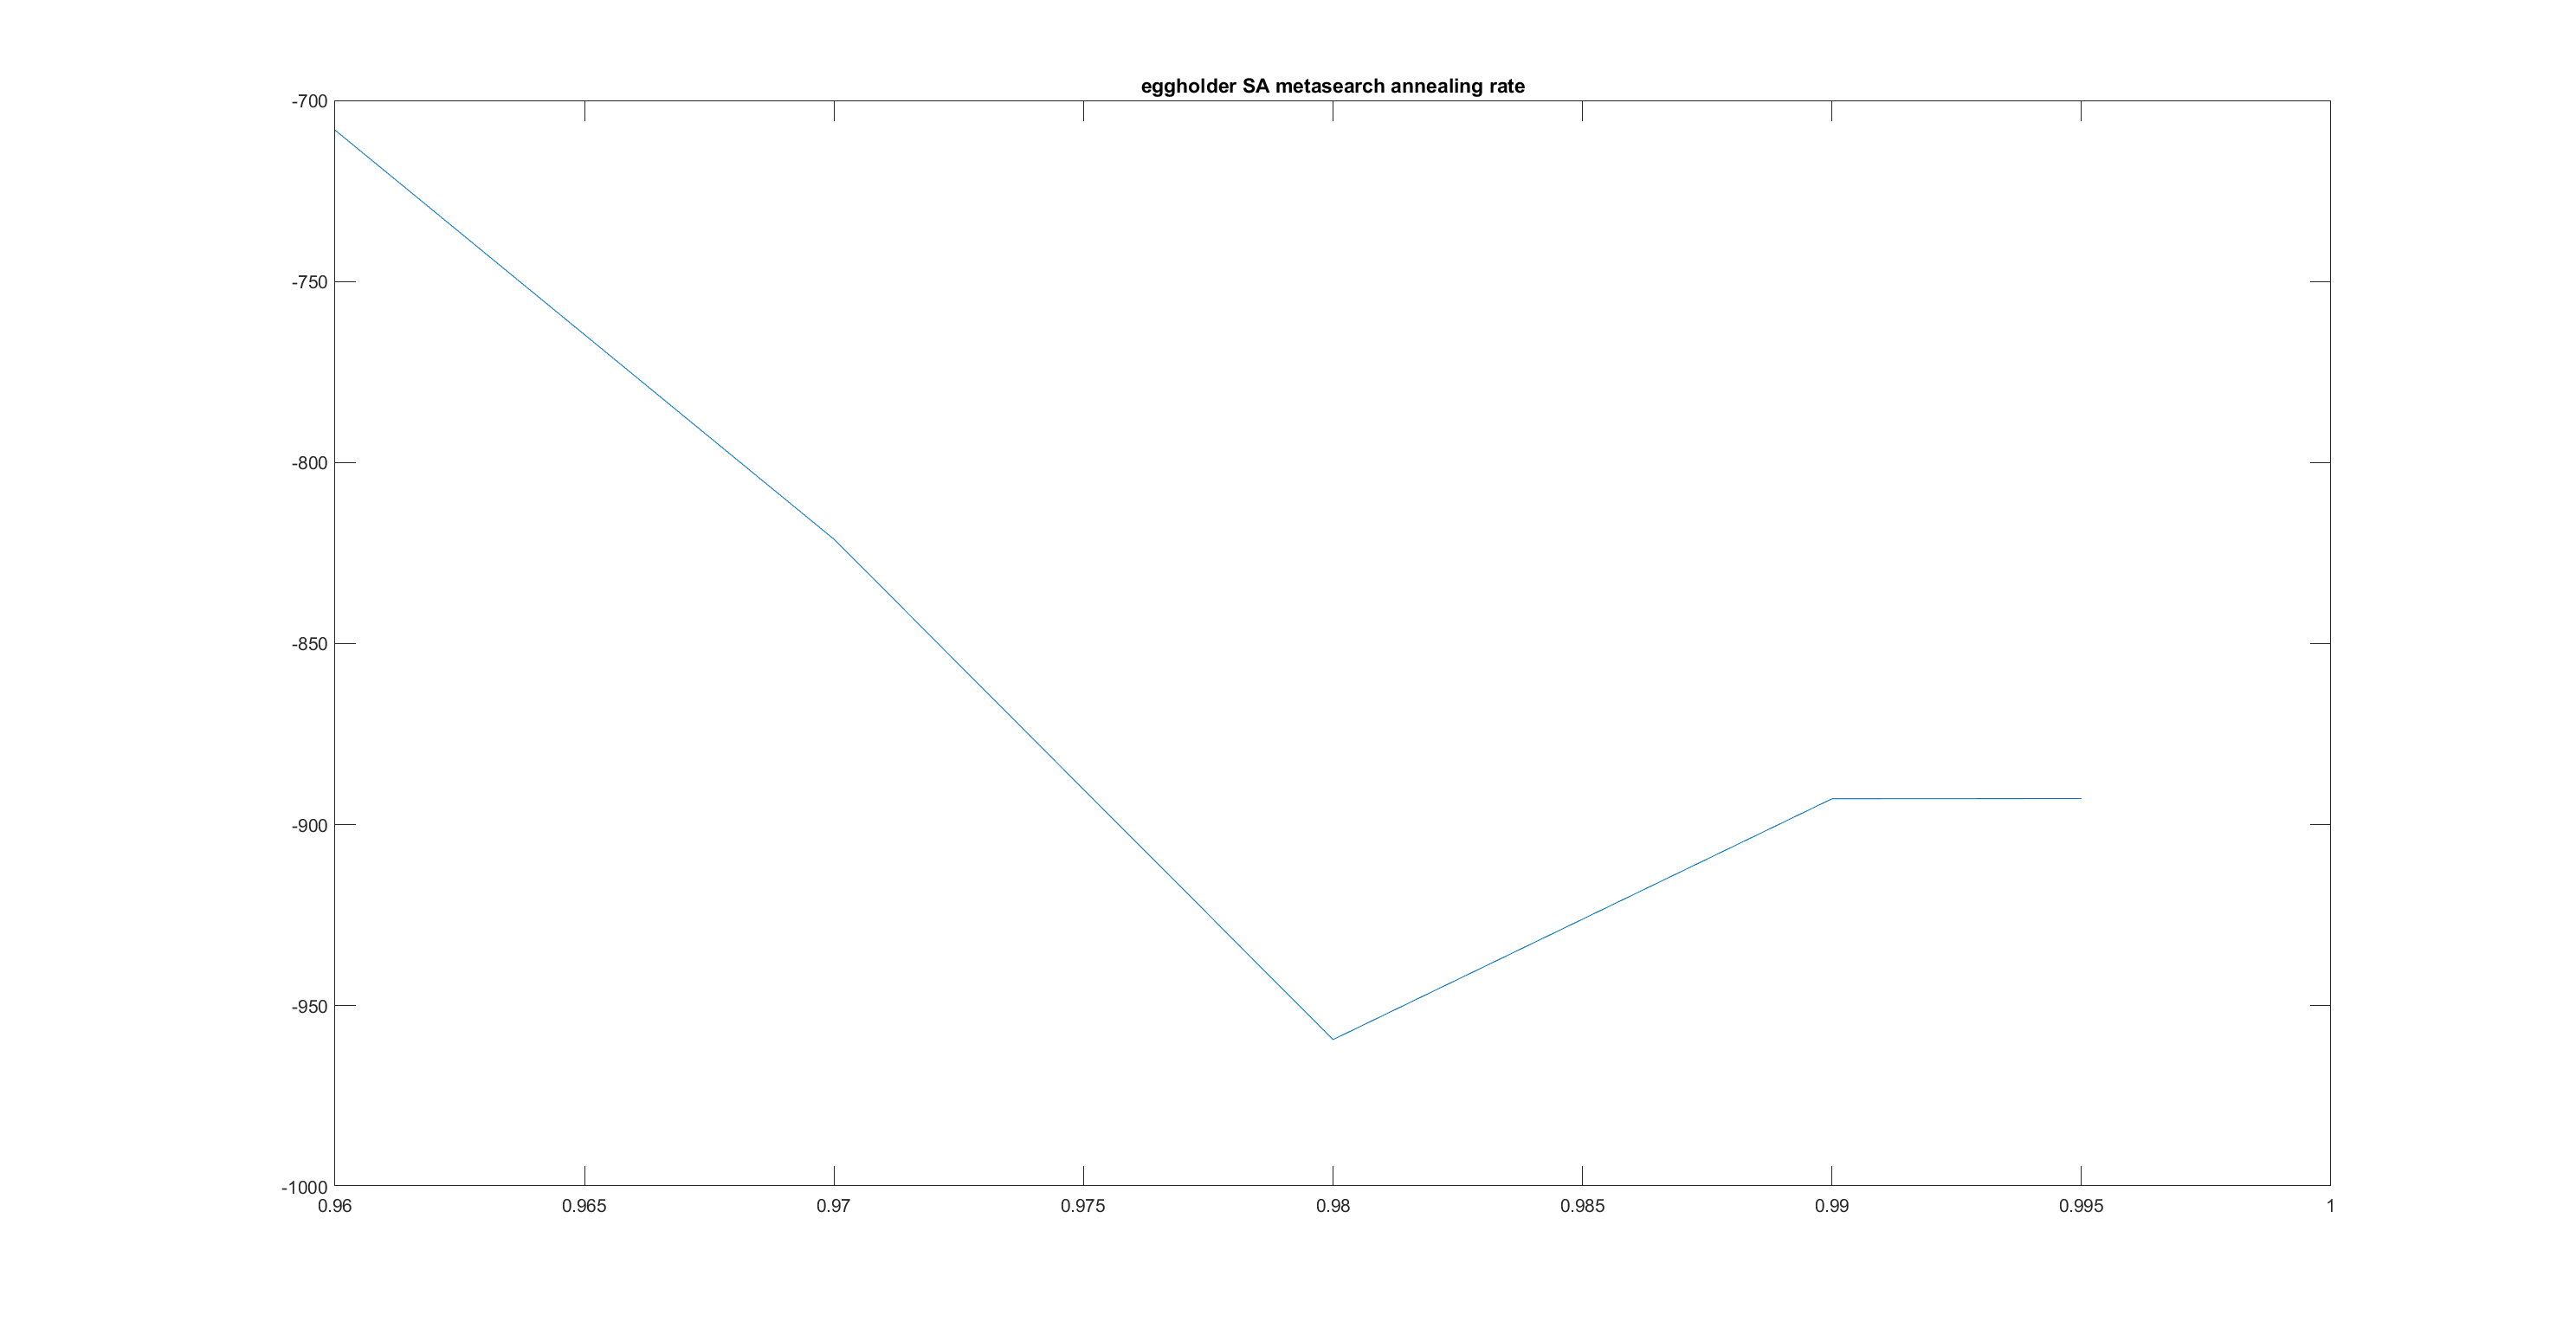
\includegraphics[width=0.45\textwidth]{Q1/figures/eggholder_SA_metasearch_annealing_rate.png}
            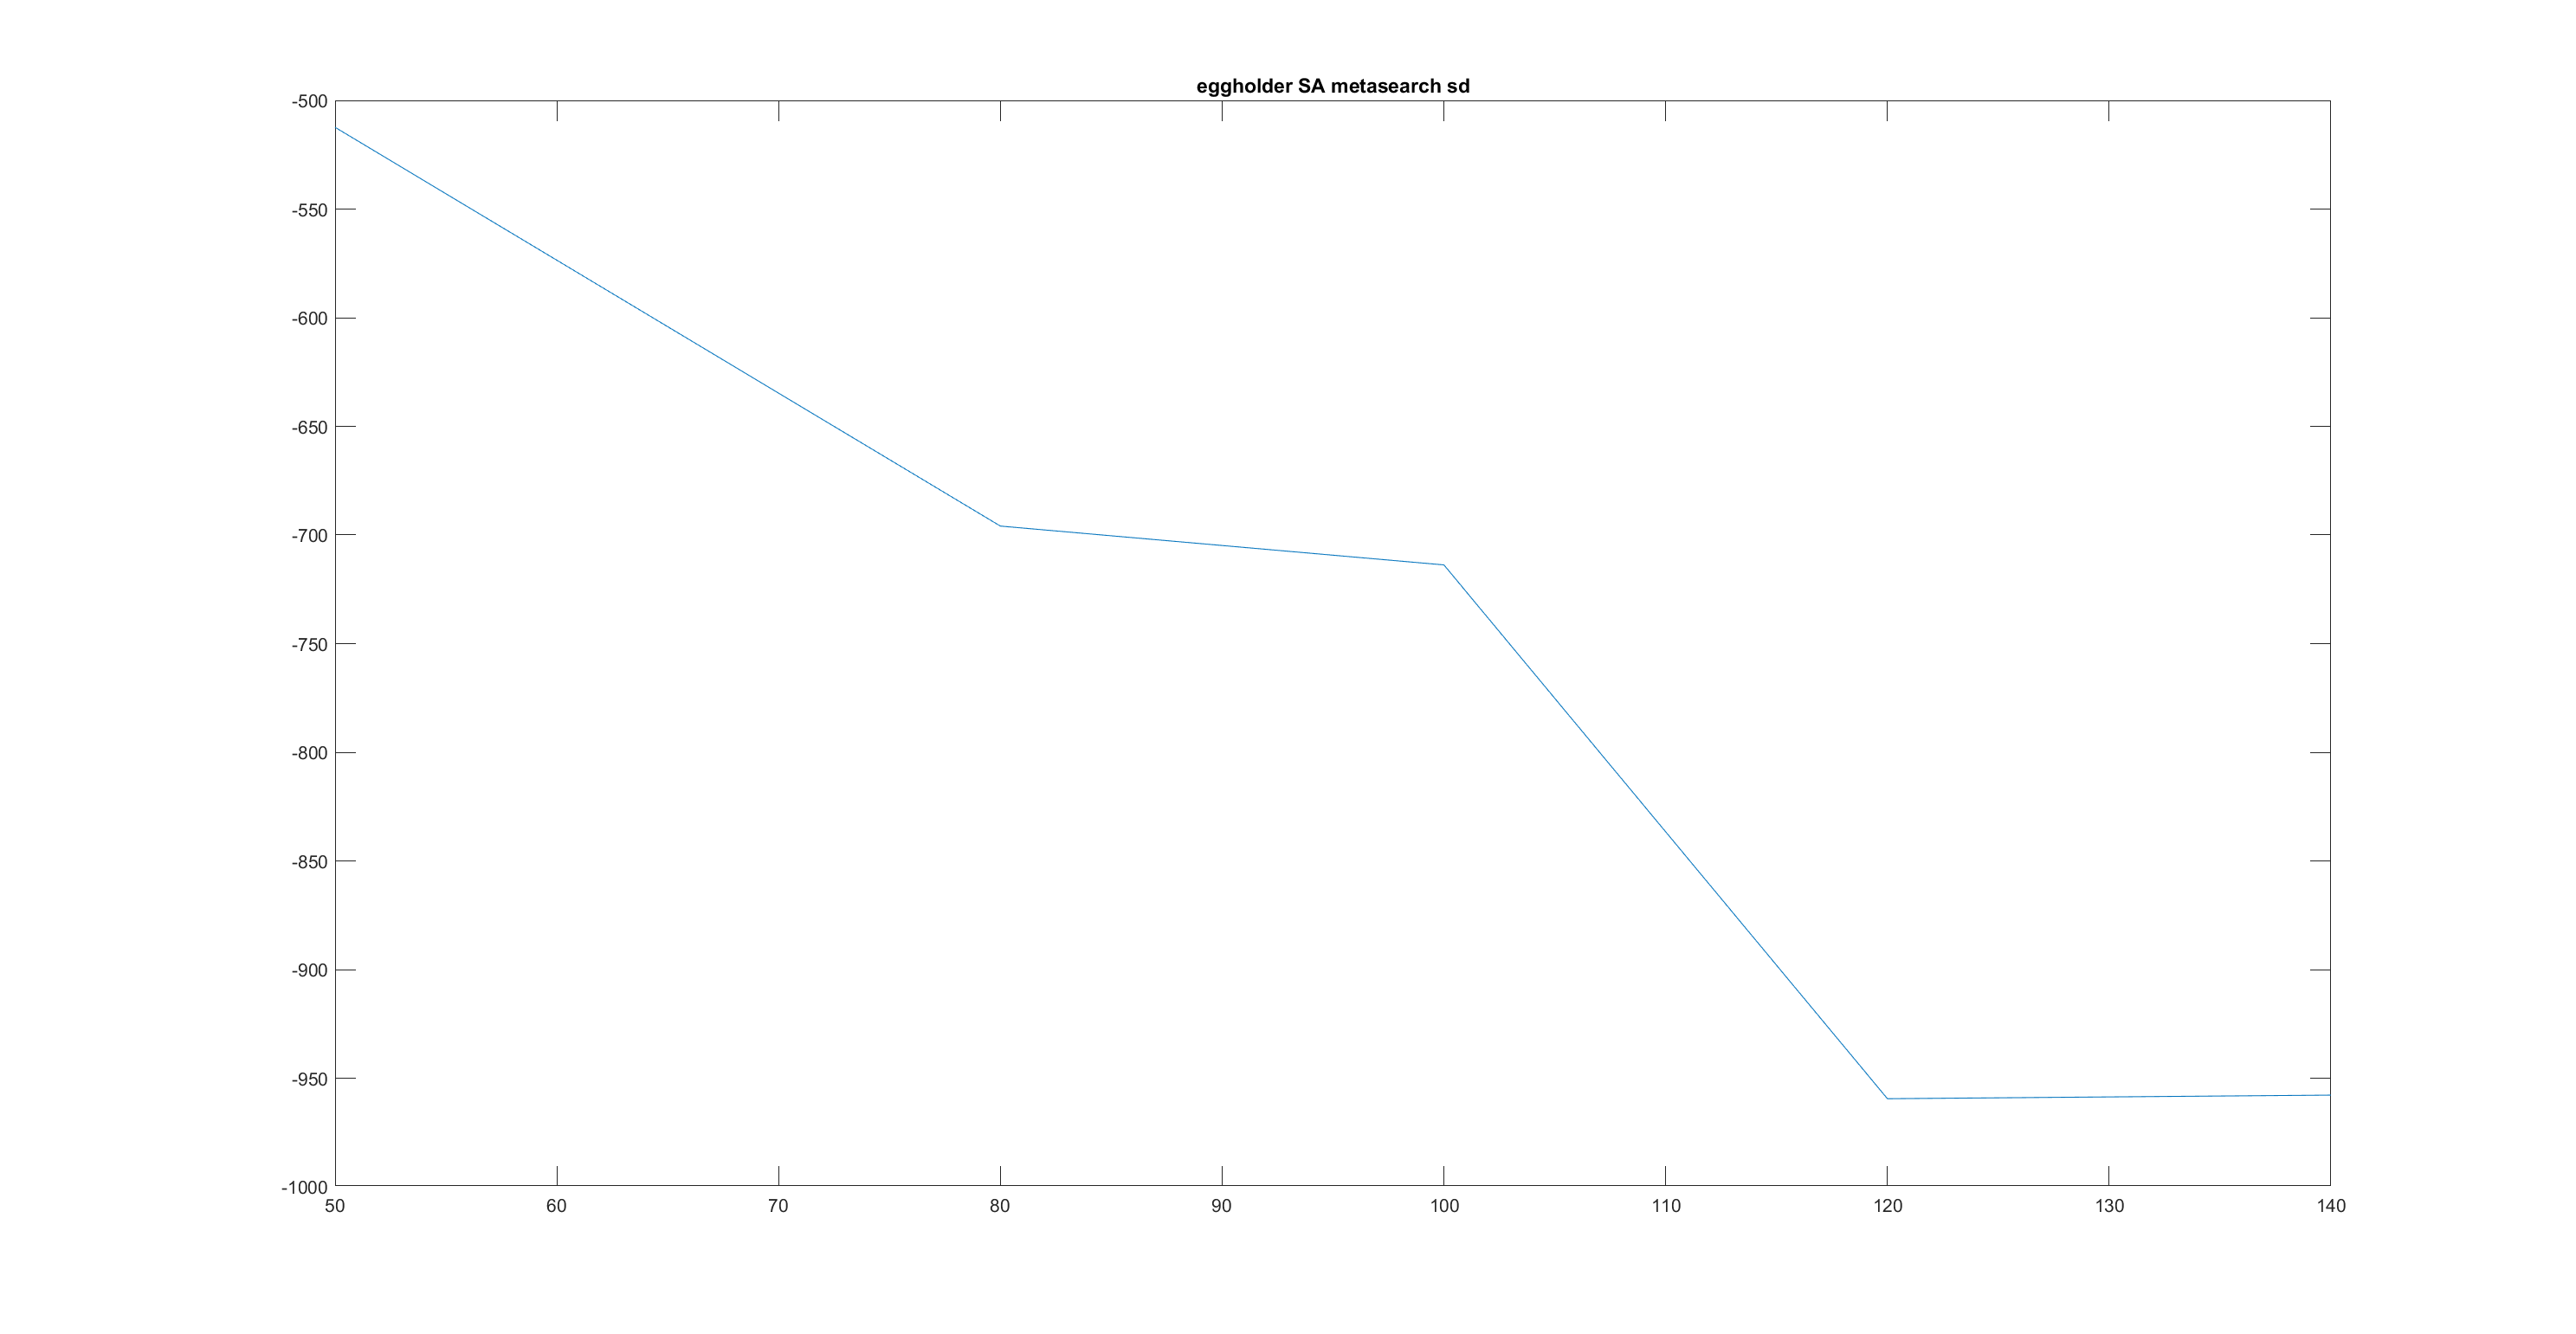
\includegraphics[width=0.45\textwidth]{Q1/figures/eggholder_SA_metasearch_sd.png}
            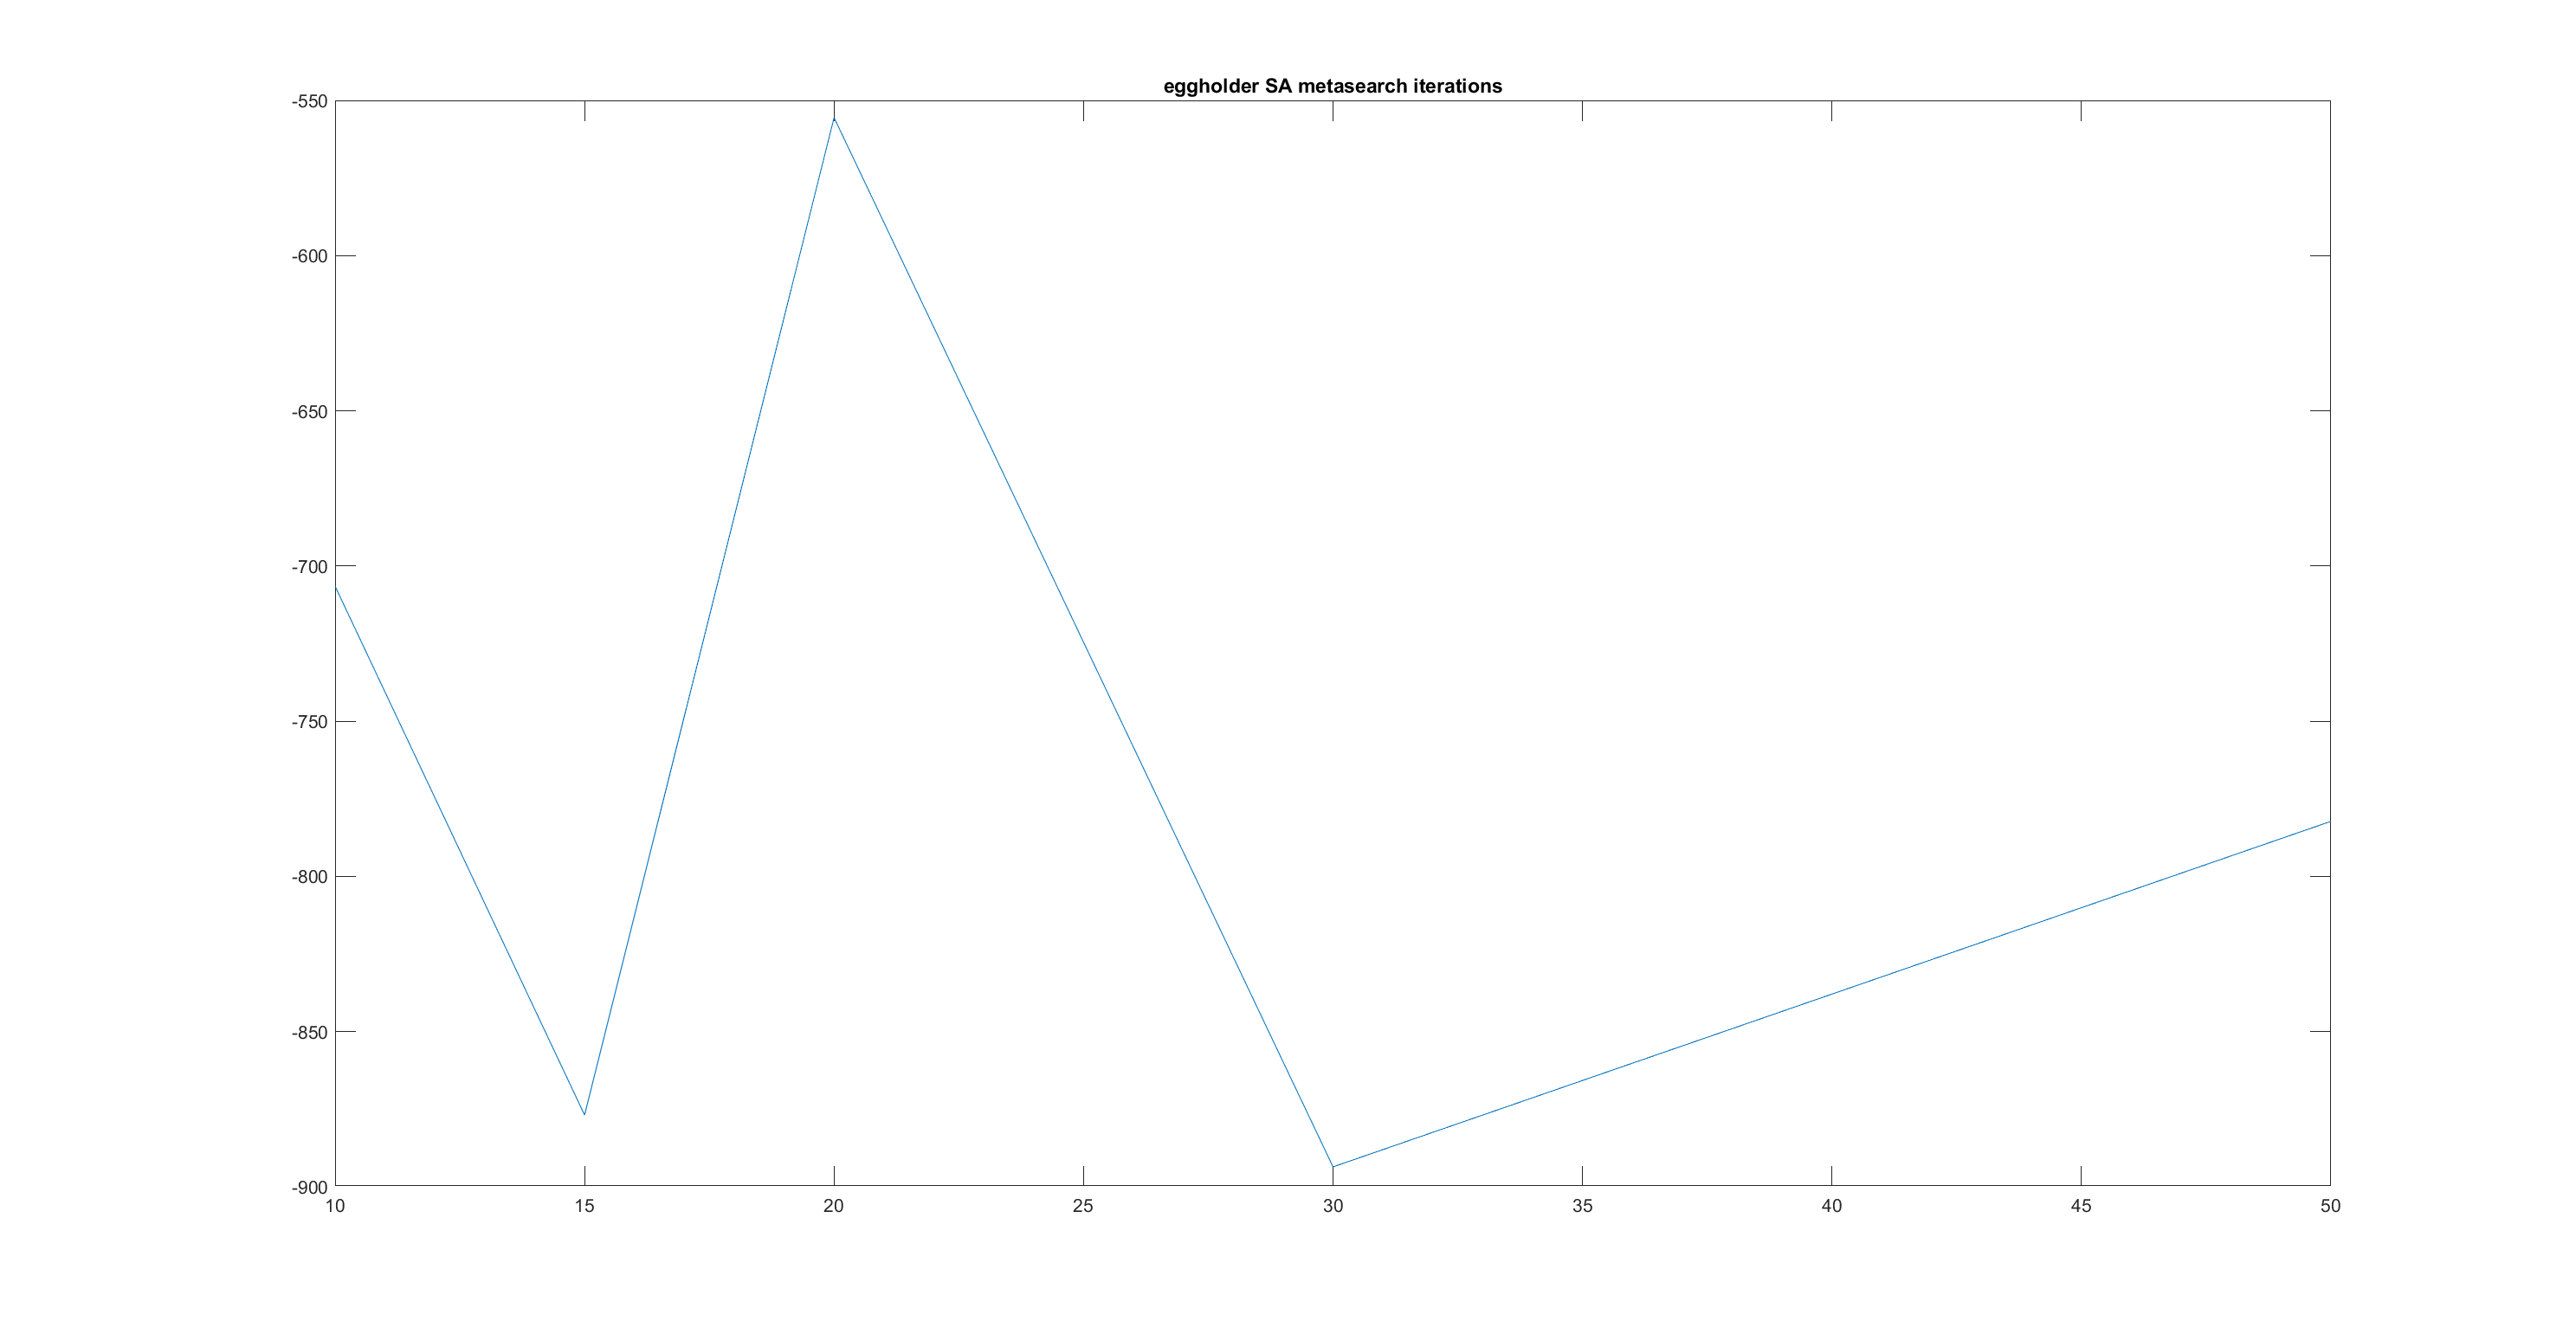
\includegraphics[width=0.45\textwidth]{Q1/figures/eggholder_SA_metasearch_iterations.png}
            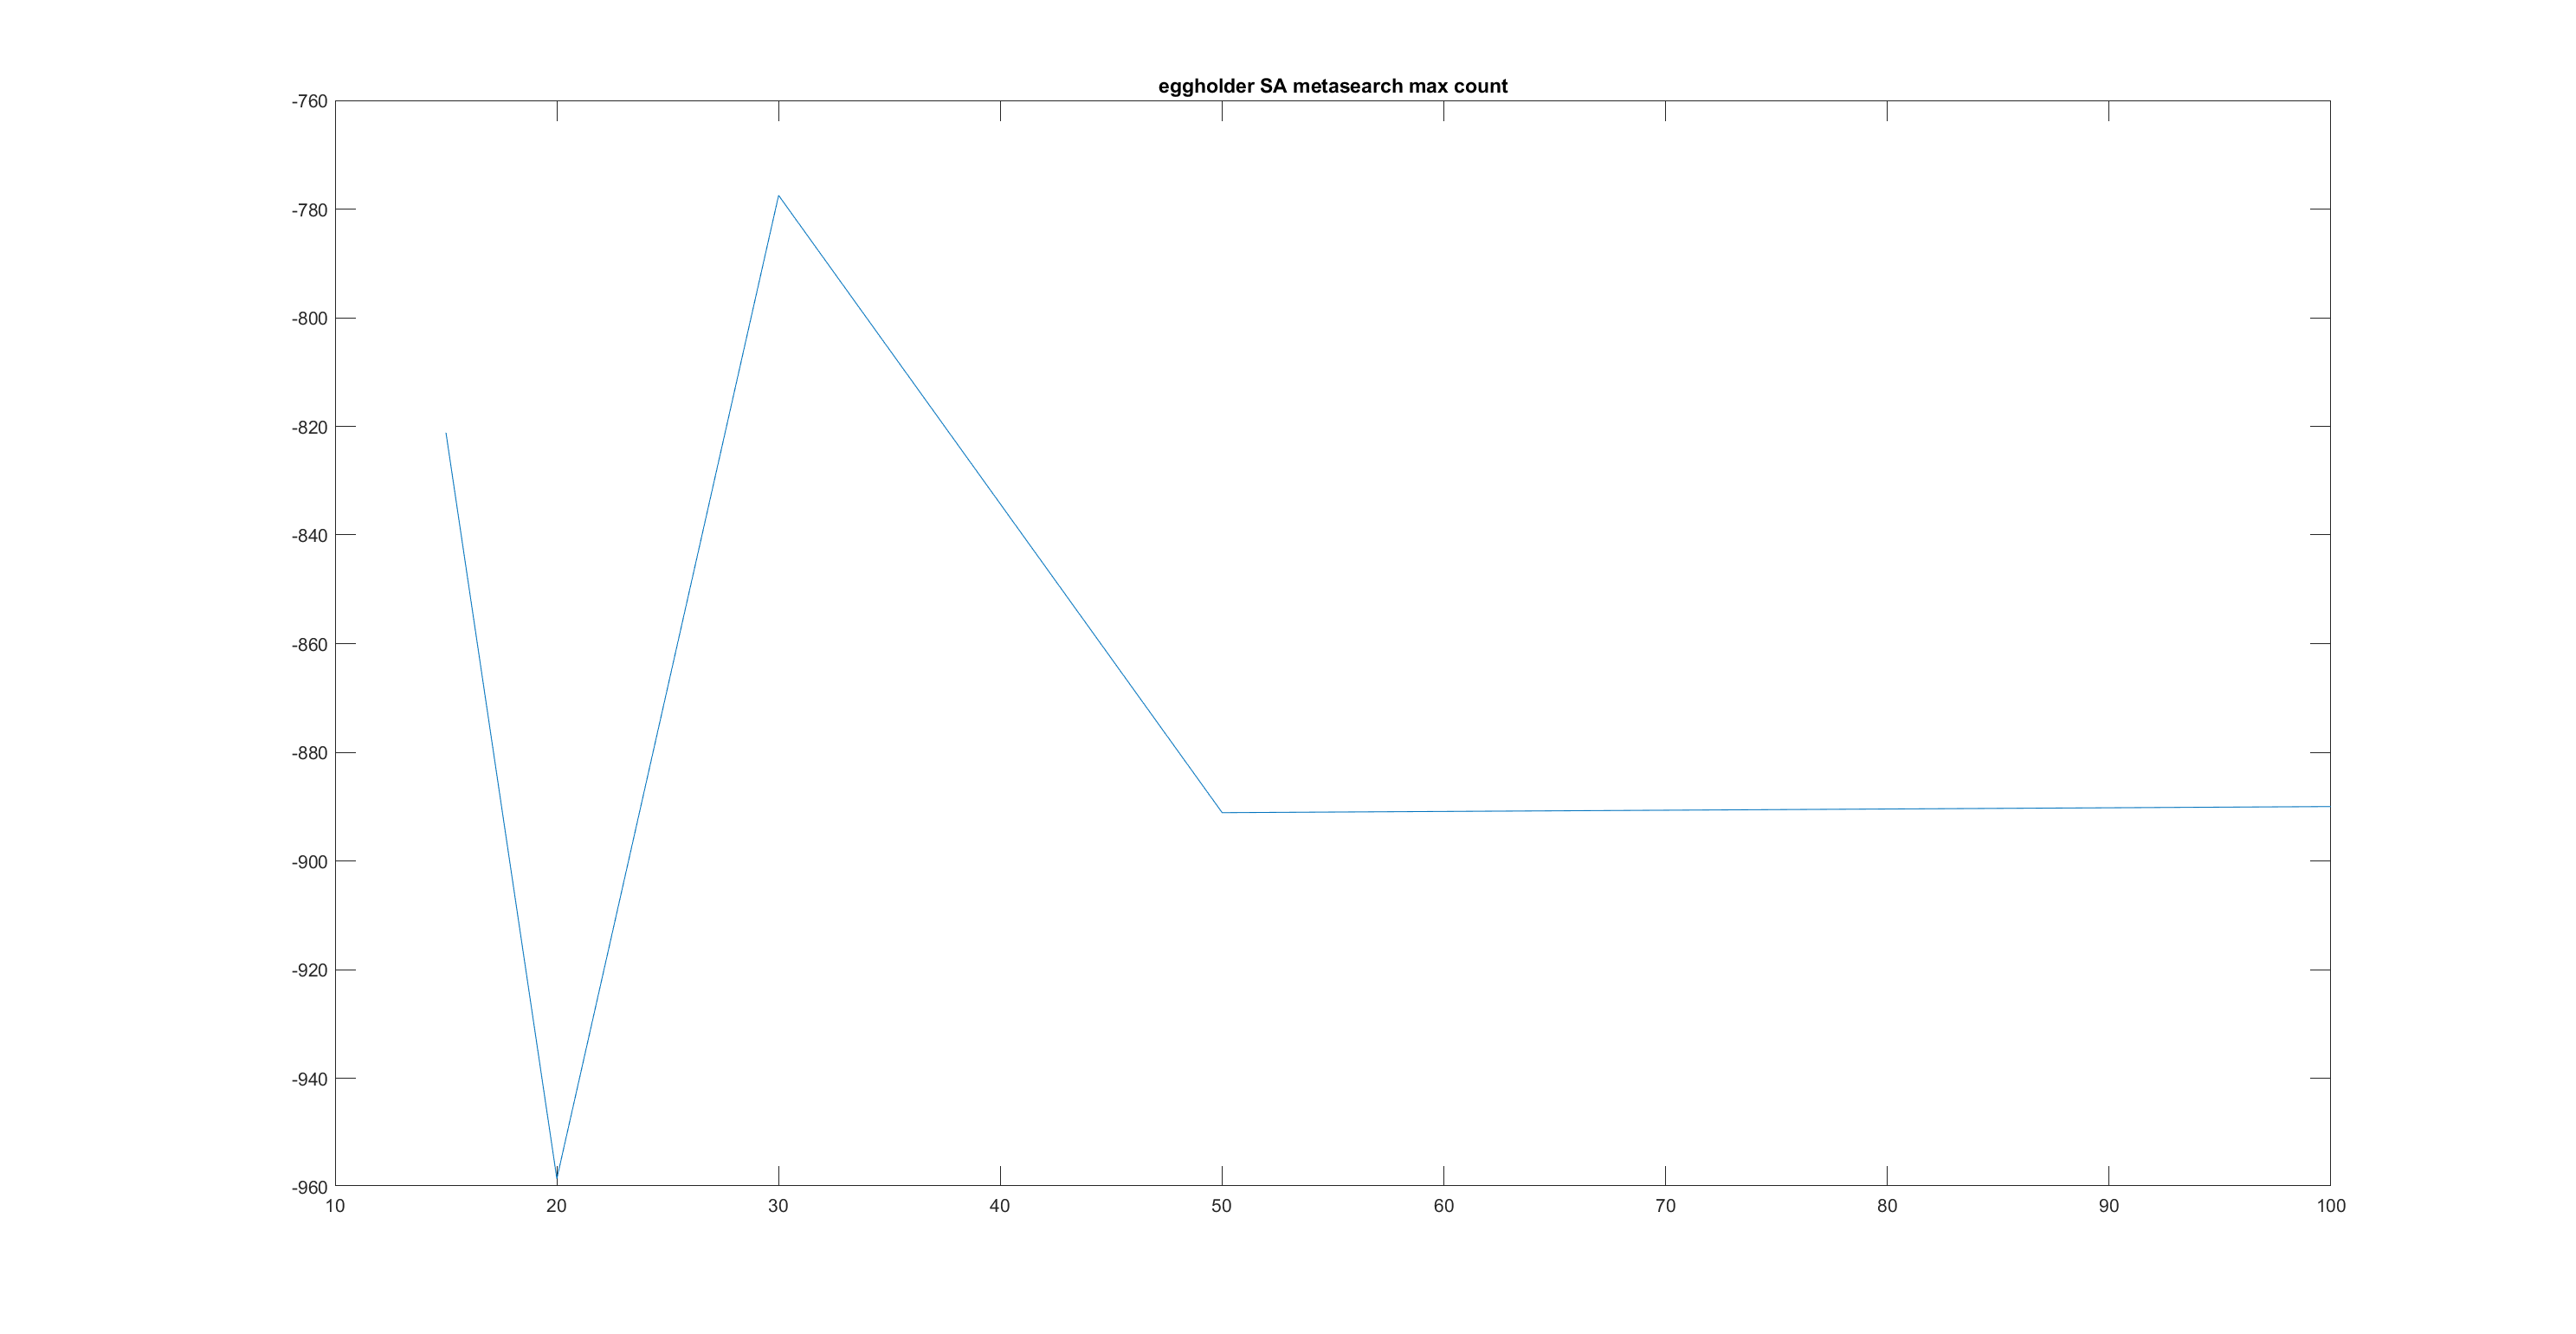
\includegraphics[width=0.45\textwidth]{Q1/figures/eggholder_SA_metasearch_max_count.png}
            \caption{Greedy sensitivity analysis for SA}
            \label{fig:sensitivity_SA}
        \end{figure}

        \begin{figure}[!htbp]
            \centering
            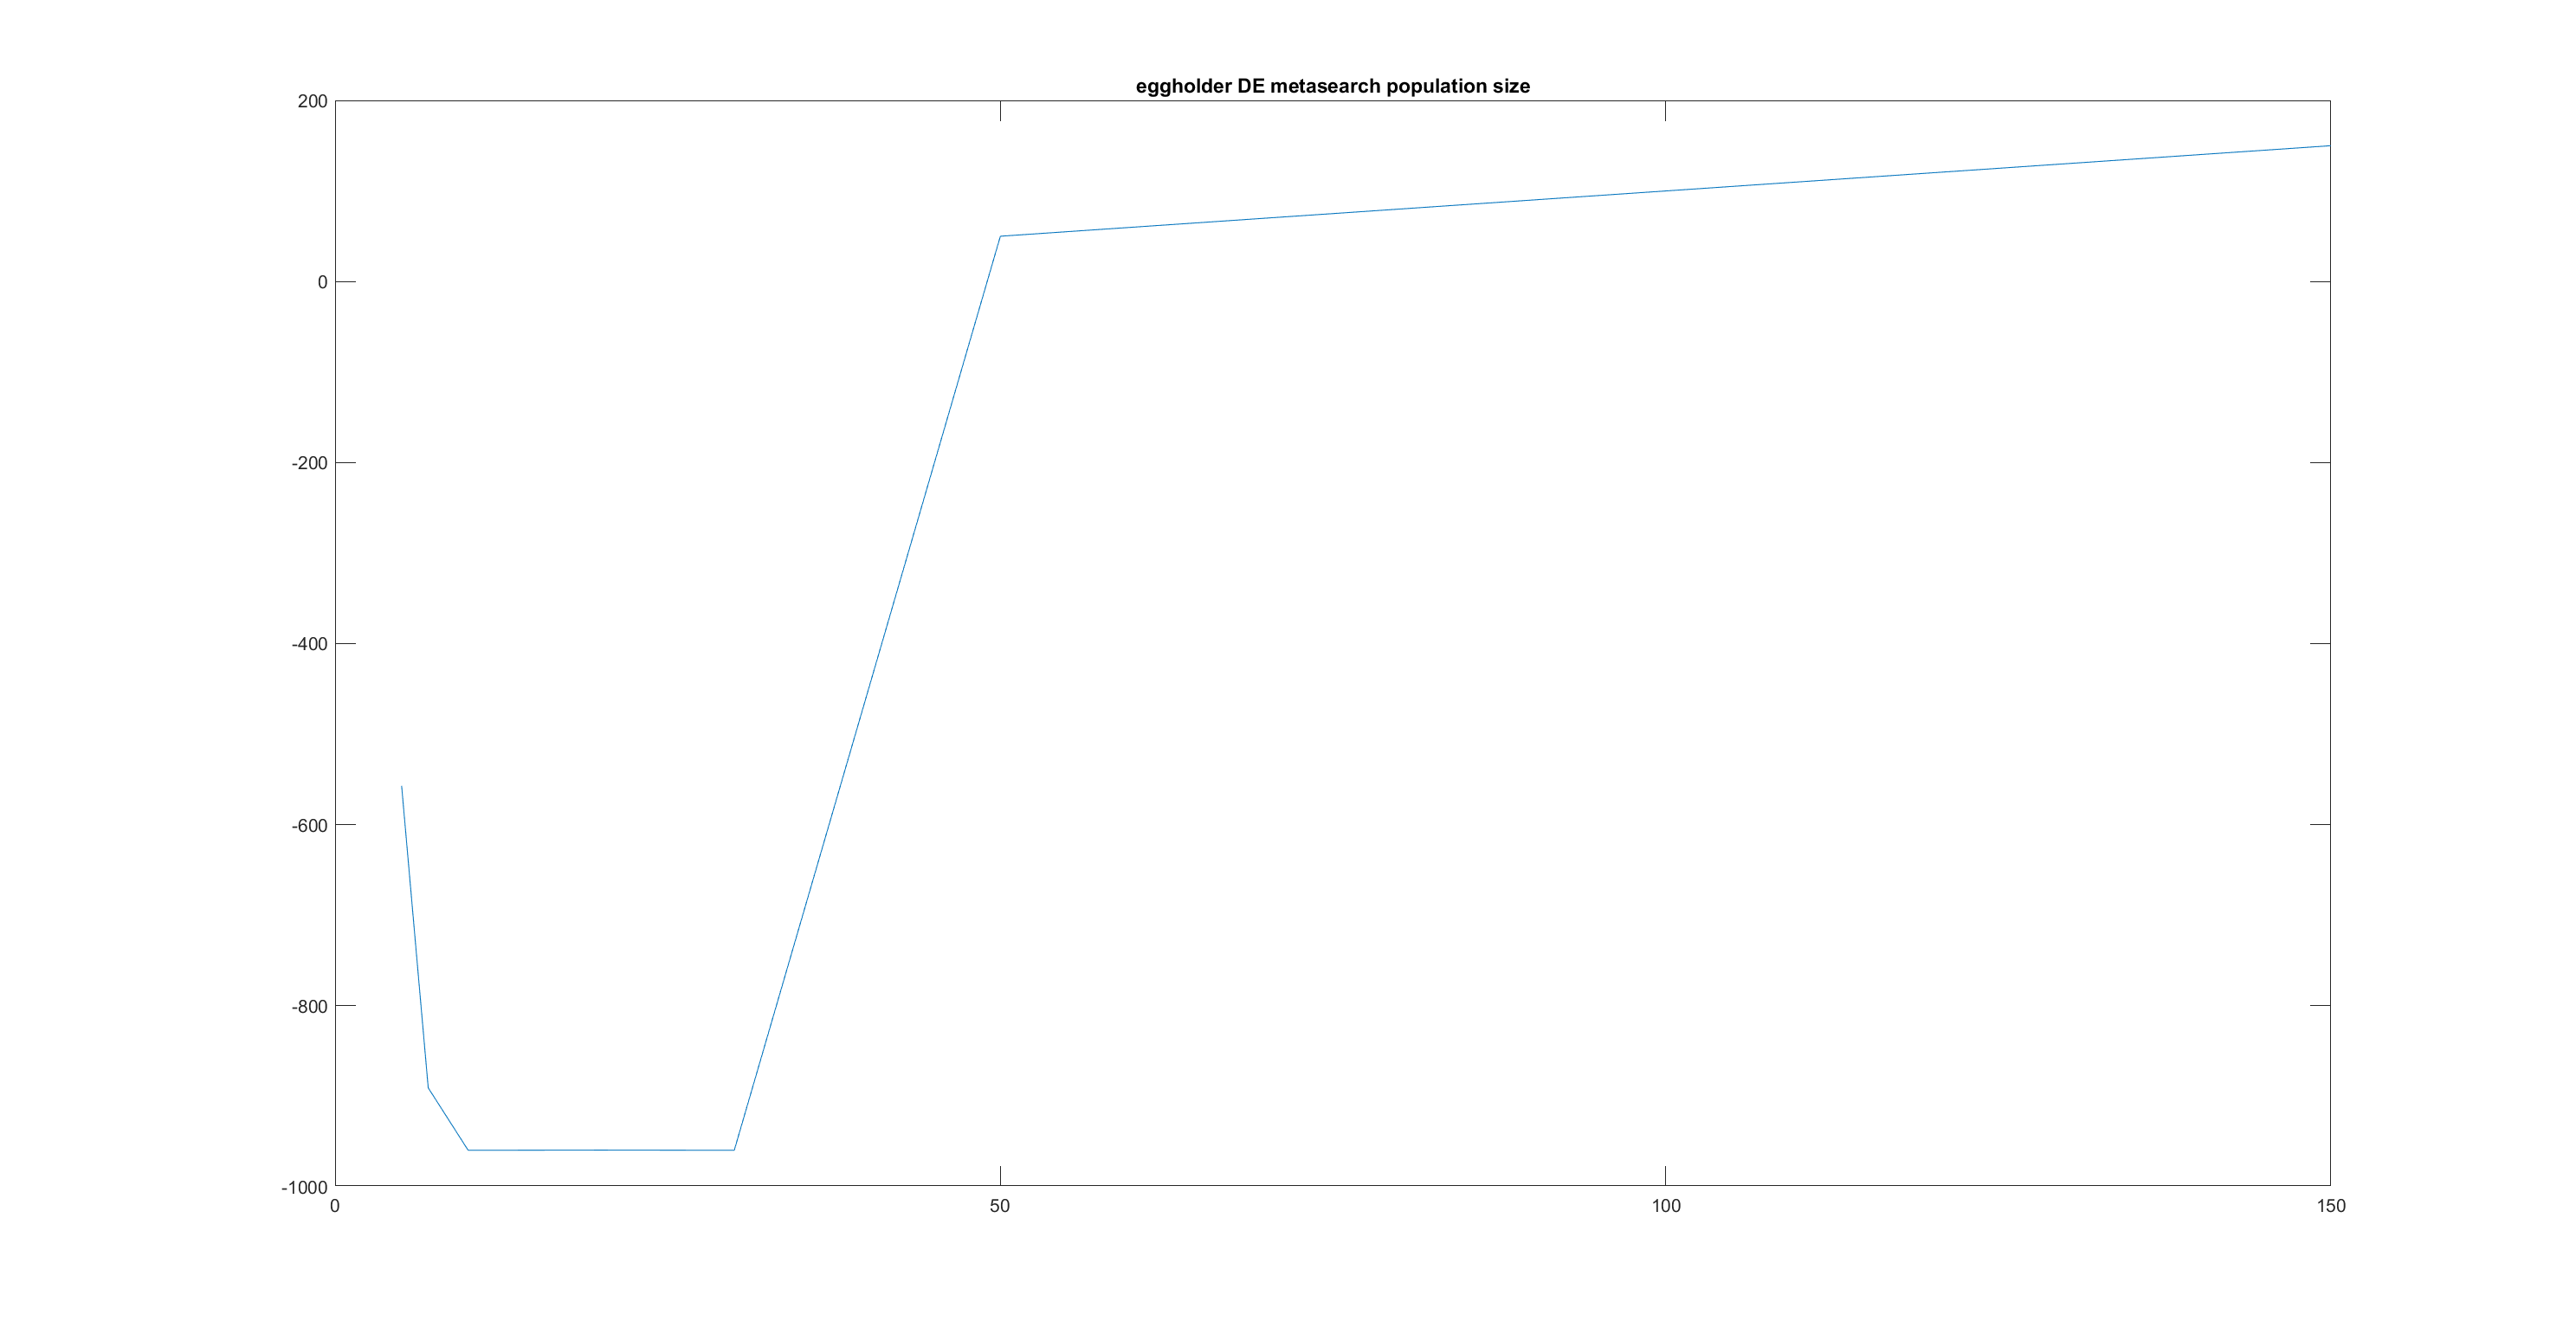
\includegraphics[width=0.45\textwidth]{Q1/figures/eggholder_DE_metasearch_population_size.png}
            \caption{Greedy sensitivity analysis for DE}
            \label{fig:sensitivity_DE}
        \end{figure}

        From Figure \ref{fig:sensitivity_SA}, we find that SA is sensitive to hyperparameters, especially initial temperature and annealing rate.
        This can be easily interpreted: the temperature determines which side the balance to fall between exploitation and exploration. 
        Luckily, the annealing rate we chose is appropriate among other four choices.
        Other hyperparametrs also count. 
        For example, the standard deviation (std.) of the Gaussian proposal function also plays a role in the balance between exploitation and exploration.

        From Figure \ref{fig:sensitivity_DE}, we see that DE depends on the population size. 
        It works fine with a population size smaller than 40. 
        With a size of 100, it needs more iterations to explore.
        If the iteration number is fixed, DE will suffer lack of exploration, which is also called ``prematurity''.
        
    }
}

\section{Question 2: Combinatorial Optimization}
{
    \subsection{Benchmark Problem: 50-city TSP}
    {
        The benchmark problem is a TSP of 50 cities. The best result known is 427.855 \cite{book:wang}. 
    }

    \subsection{Experiment}
    {
        Repeated for 20 times, the performance (best value searched and time cost) of each algorithm is recorded. 
        (Table \ref{tab:performance_Q2} and \ref{tab:timecost_Q2})
        (Figure \ref{fig:TSP_SA})

        \begin{table}[!hbp]
            \centering
            \begin{tabular}{|c|c|c|c|}
                \hline
                Alg. & best so far (min) & b.s.f. (mean) & b.s.f. (max) \\
                \hline
                SA &  438.7710 &  472.3798 &  493.6293 \\
                \hline
            \end{tabular}
            \caption{Performance after 20th repitition}
            \label{tab:performance_Q2}
        \end{table}

        \begin{table}[!hbp]
            \centering
            \begin{tabular}{|c|c|c|c|}
                \hline
                Alg. & time cost in sec (min) & t.c. (mean) & t.c. (max) \\
                \hline
                SA &  312.9063 &  341.9633 &  398.1719 \\
                \hline
            \end{tabular}
            \caption{Time cost after 20th repitition}
            \label{tab:timecost_Q2}
        \end{table}
        
        \begin{figure}[!htbp]
            \centering
            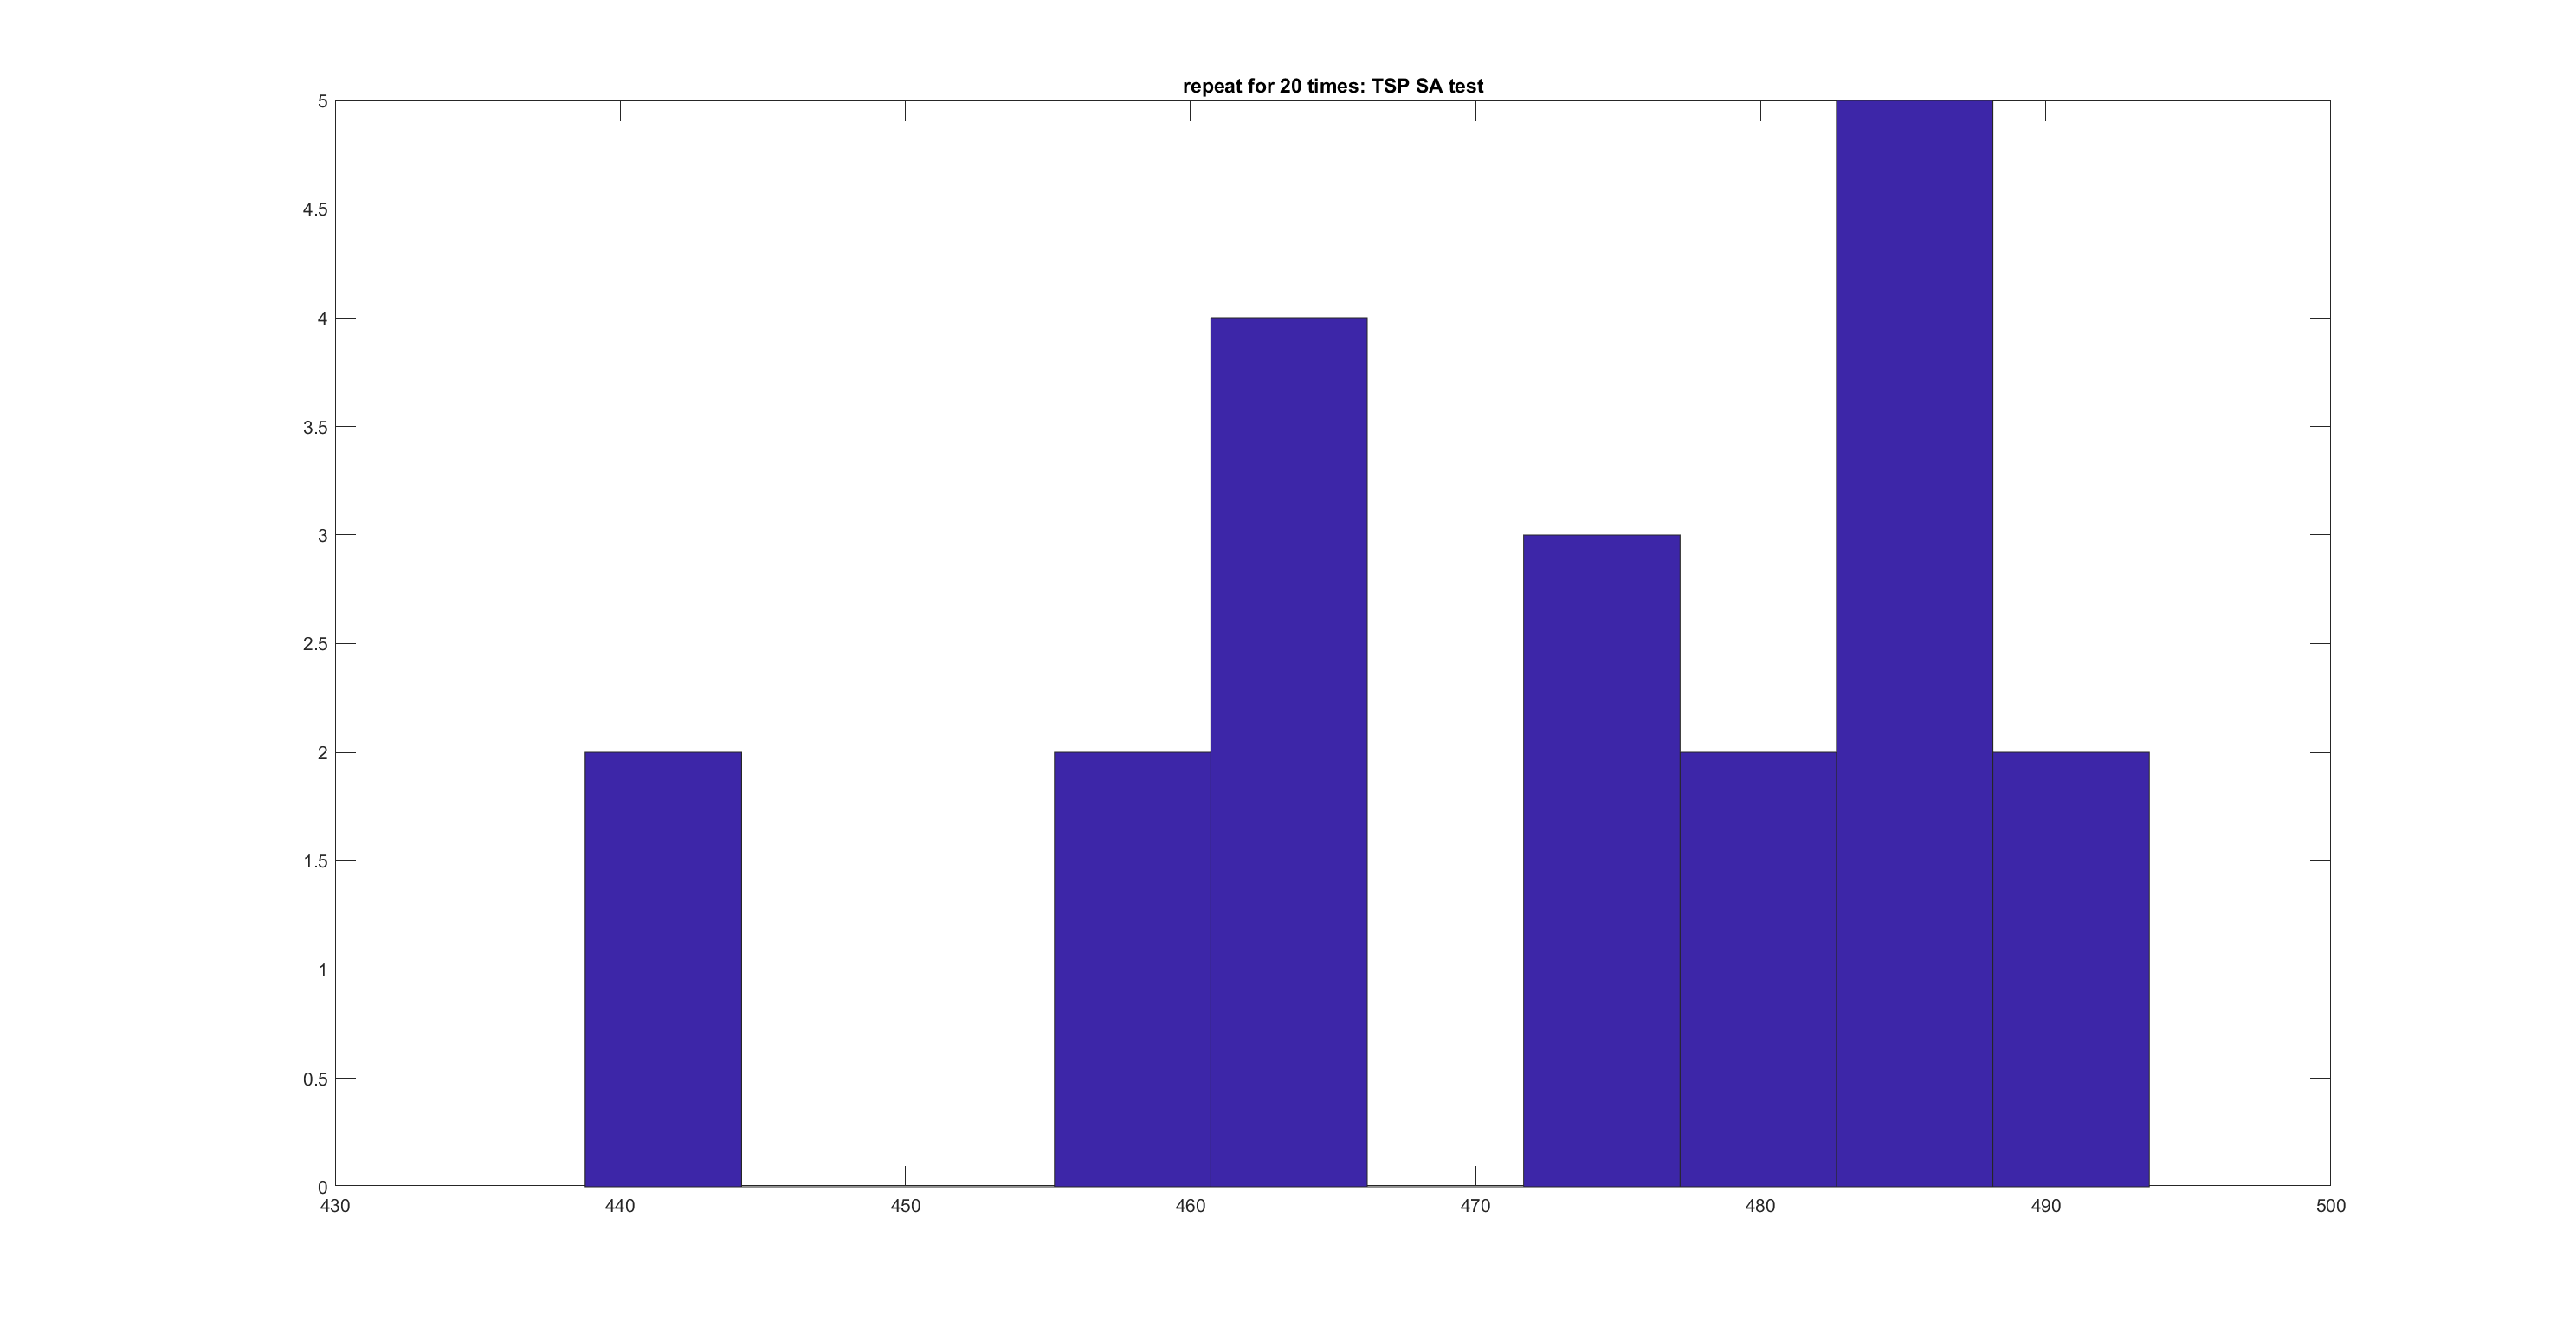
\includegraphics[width=0.45\textwidth]{Q2/figures/TSP_SA_test.png}
            \caption{Performance of SA after 20th repitition}
            \label{fig:TSP_SA}
        \end{figure}

        Compared with the best result known, 427.855, the simulated annealing achieves similar performance in the best case.
        The worst case is also acceptable in most cases. 
        The time cost, however, is very high because too many iterations are needed before it could converge.
    }

    \subsection{Discussion}
    {
        For the 10th experiment (Figure \ref{fig:TSP_SA_example}), we see that the simulated annealing converges slowly. 
        At first, exploration outweights exploitation as the temperature is high and therefore worse results are more likely to be accepted.
        As the temperature decreases, exploitation is more and more preferred, making the process converge and halt.

        \begin{figure}[!htbp]
            \centering
            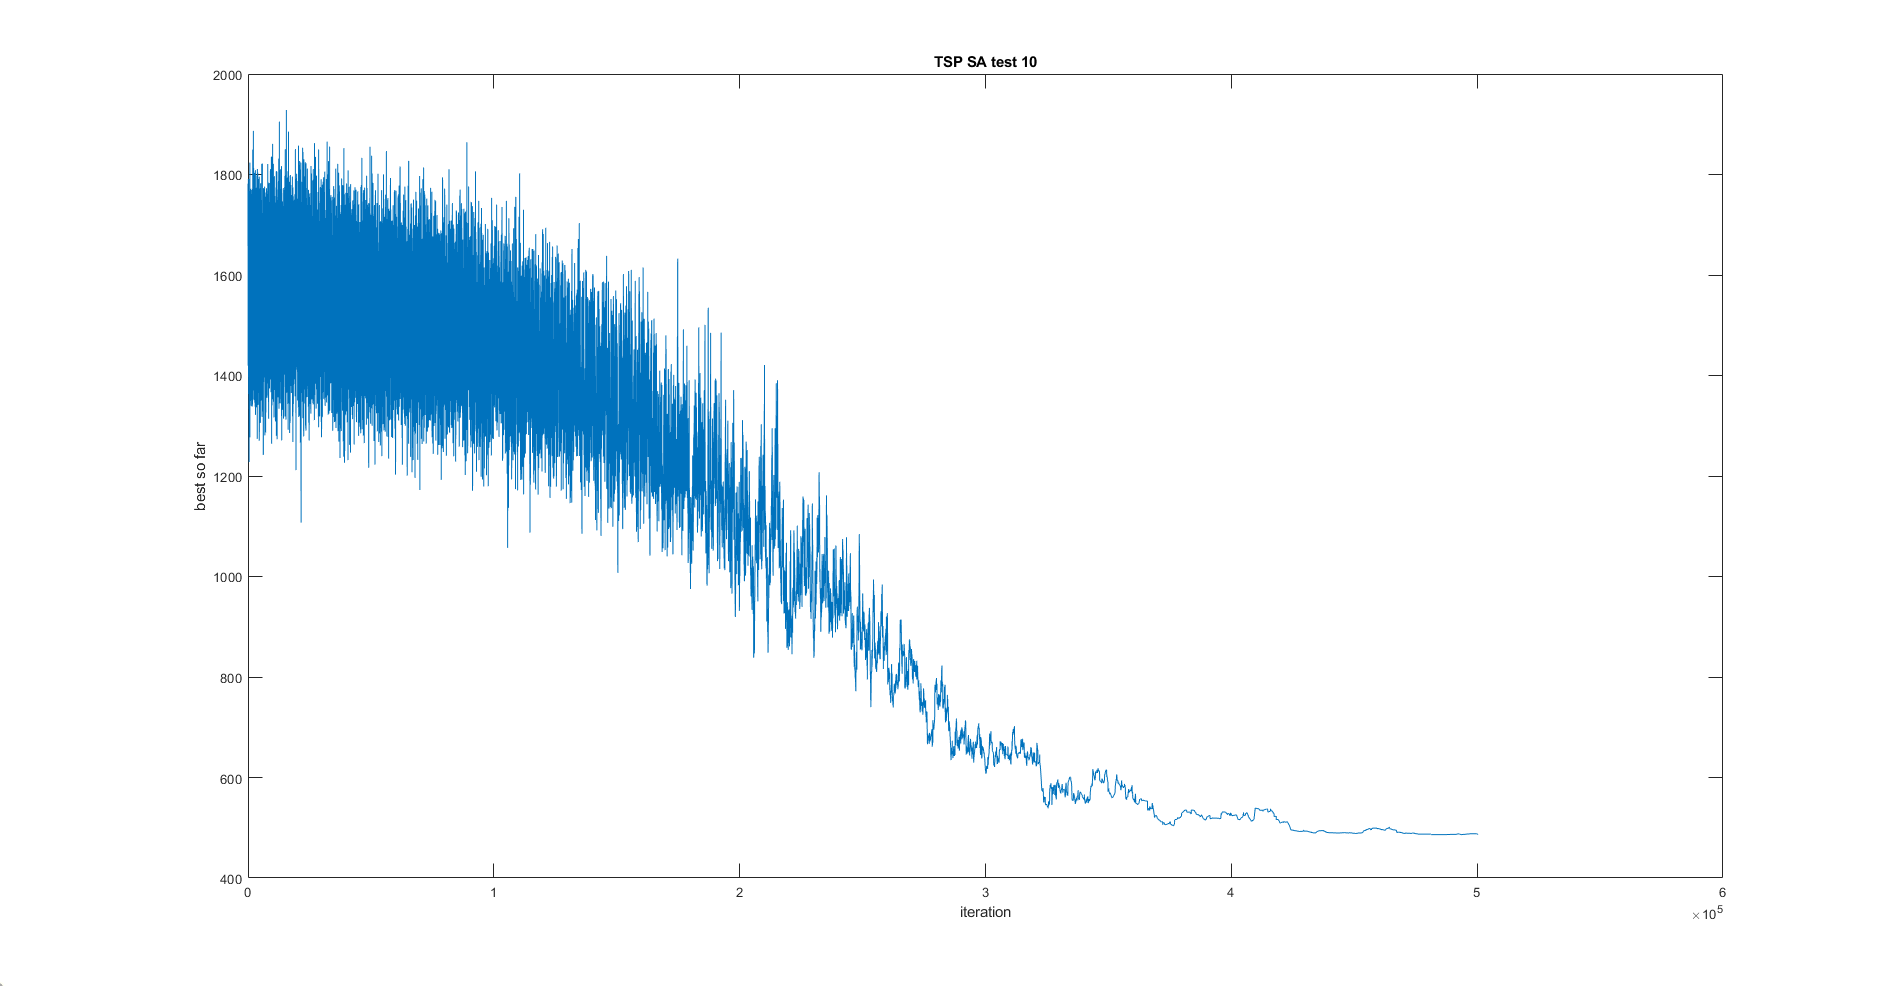
\includegraphics[width=0.45\textwidth]{Q2/figures/TSP_SA_test_result_10.png}
            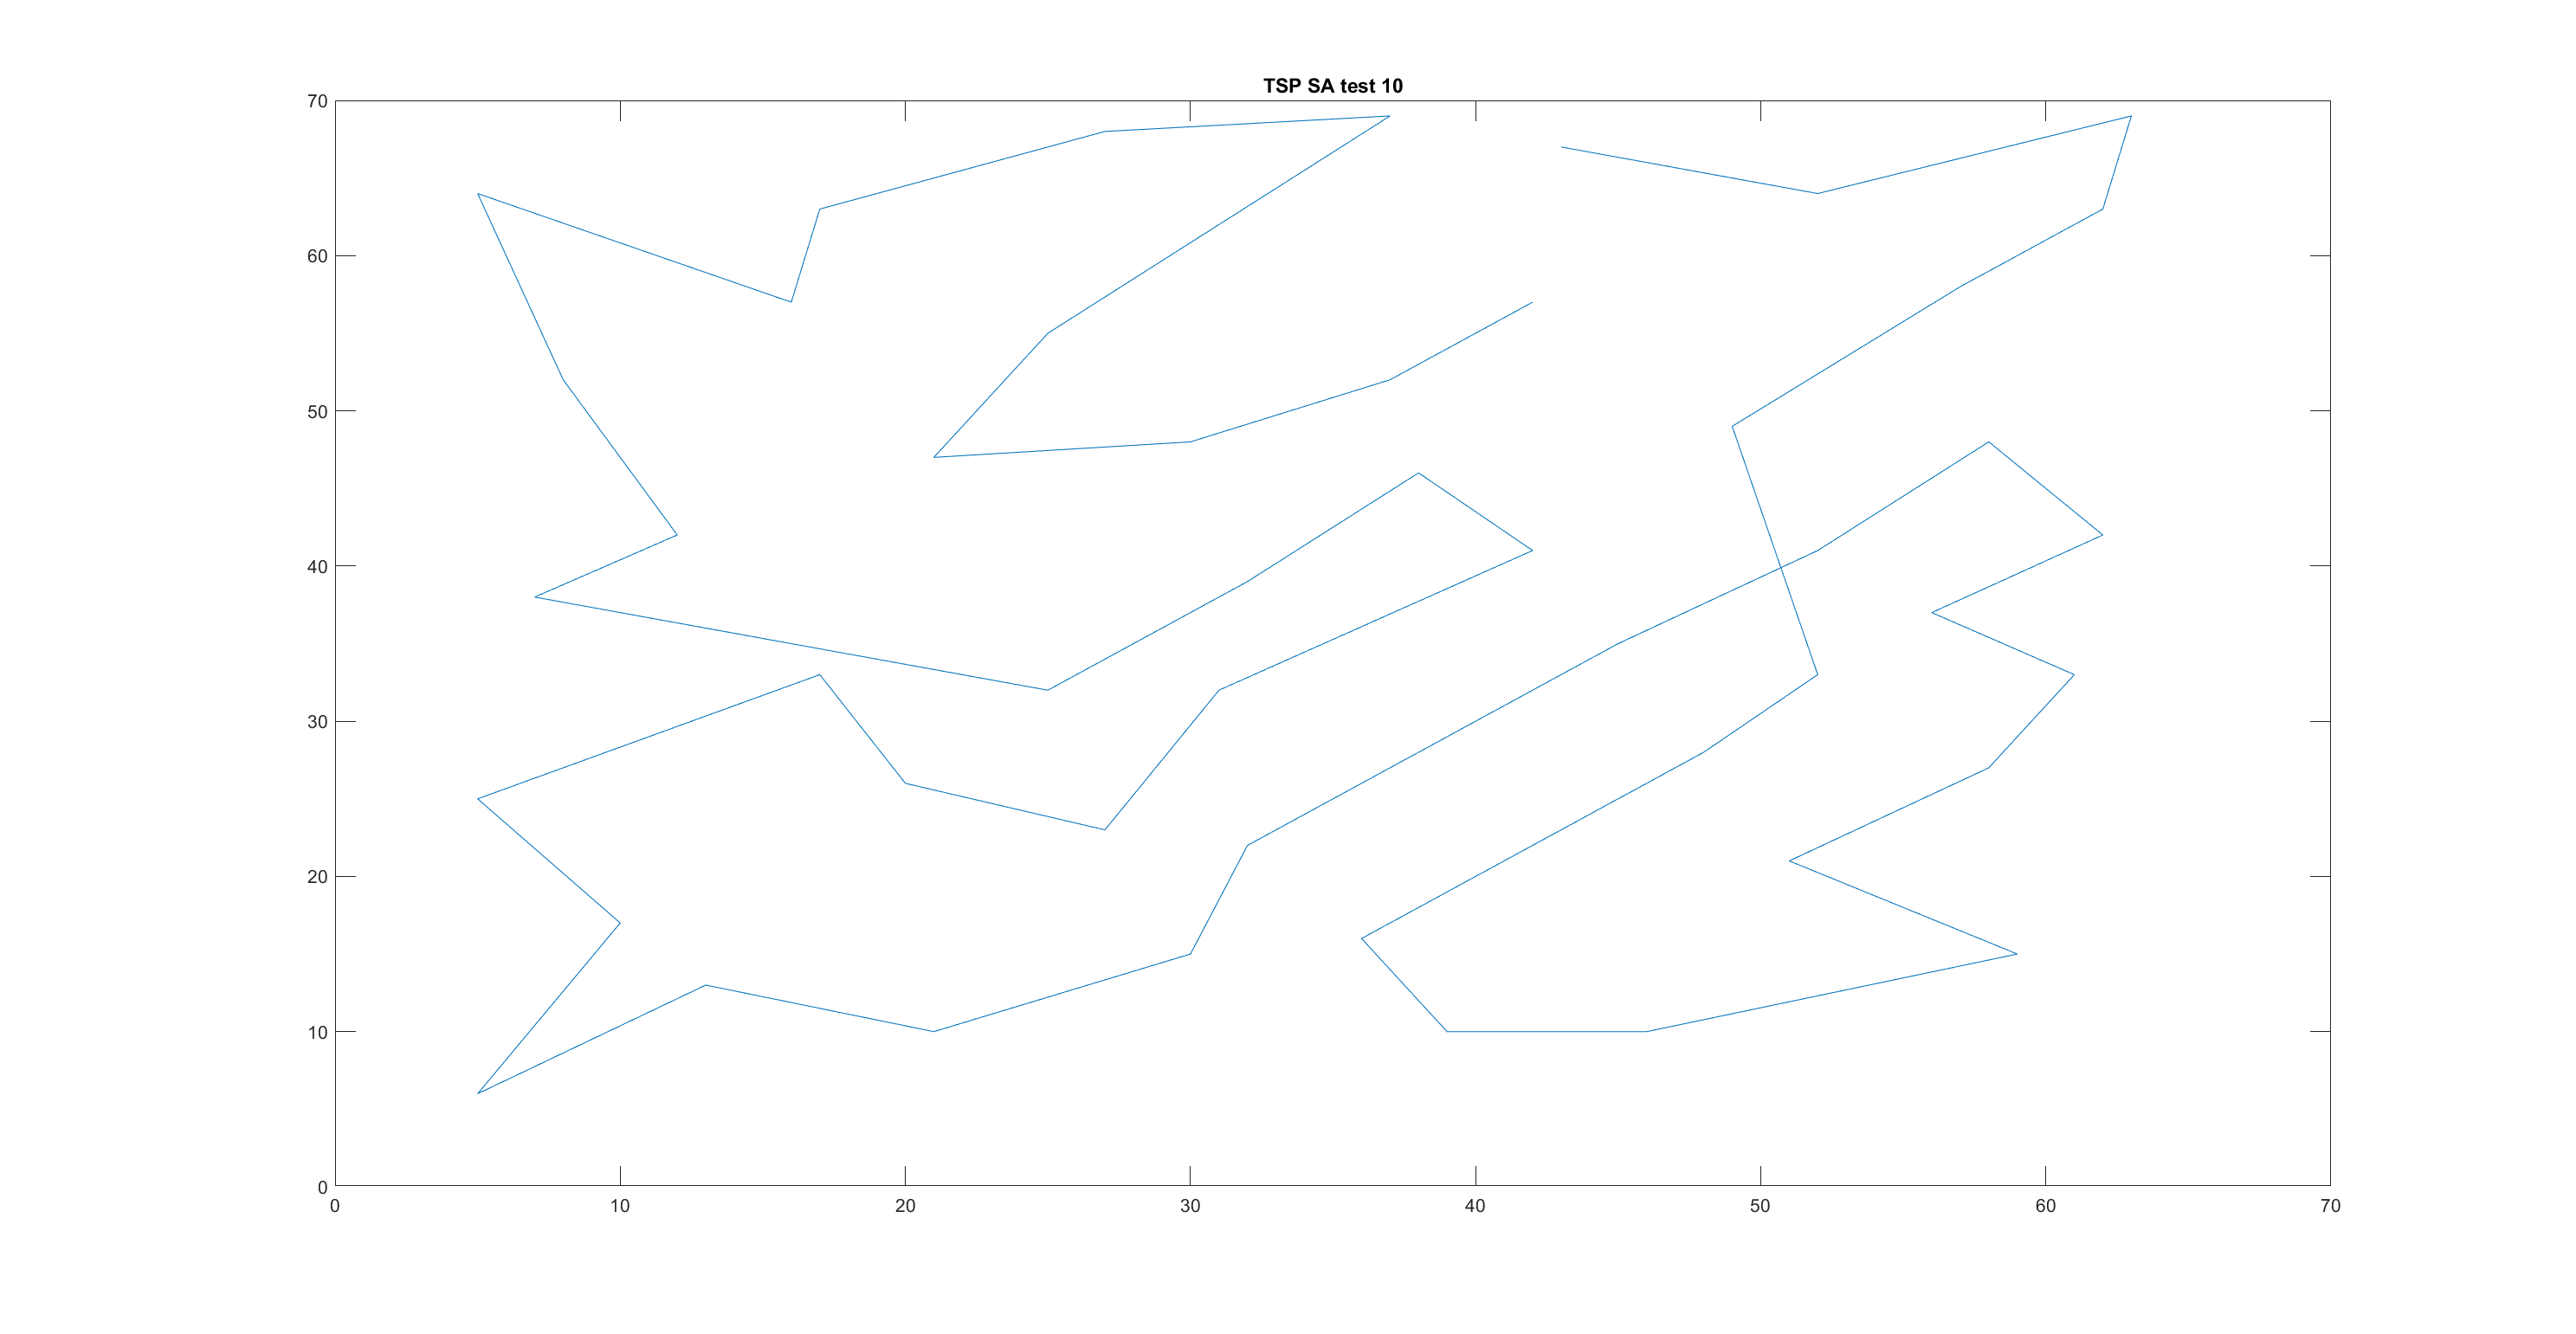
\includegraphics[width=0.45\textwidth]{Q2/figures/TSP_SA_test_10.png}
            \caption{Test case \#10}
            \label{fig:TSP_SA_example}
        \end{figure}

        Here are the final remarks:
        \begin{itemize}
            \item Combinatorial optimization is usually more time-consuming than function optimization with the same size.
            This is partly due to the time cost of mutation and crossover, whereas the time cost of real number calculation is neglegible.
            \item Hyper tuning is the most tricky part in SA, particularly for the temperature. 
            While an improper annealing rate would only slower the convergence process, 
            an improper initial temperature could impede convergence from the very beginning.
            I tried different initial temperatures of a geometric series, ranging from 0.01, 0.1, 1, 10, 100, 1000, etc. 
            After locating the optimal initial temperature $t_0$ between 0.1 and 1, I used binary search to find the optimal one.
            I finally chose $t_0 = 0.2$.
            \item To speed up the process and add more exploration to it, I modified SA a bit:
            In my implementation, the mutation can consist of several consecutive swaps, rather than only one swap.
            I tested it and only 400,000 iterations are needed with multiple swaps, whereas they are not enough with single swap.
        \end{itemize}
    }
}

\section{Question 3: Paper Reading about Drilling Path Optimization}
{
    In a machining center, holes-machining is a typical operation. 
    For instance, the production of PCB (printed circuit board) requires an intense procedure of drilling (Figure \ref{fig:drillings}).
    The drilling process takes much time, as much as 70\% of total operation time, due to slow motion of the cutting tools. \cite{zhu2008drilling}
    Therefore, it is worth it reducing that time by finding an optimal drilling path.
    Similar to the TSP, the drilling path problem is NP-hard, and therefore intelligent optimization algorithms are needed.
    In this section, a work using swarm particle algorithms \cite{zhu2008drilling} will be summarized.
    \begin{figure}[!htbp]
        \centering
        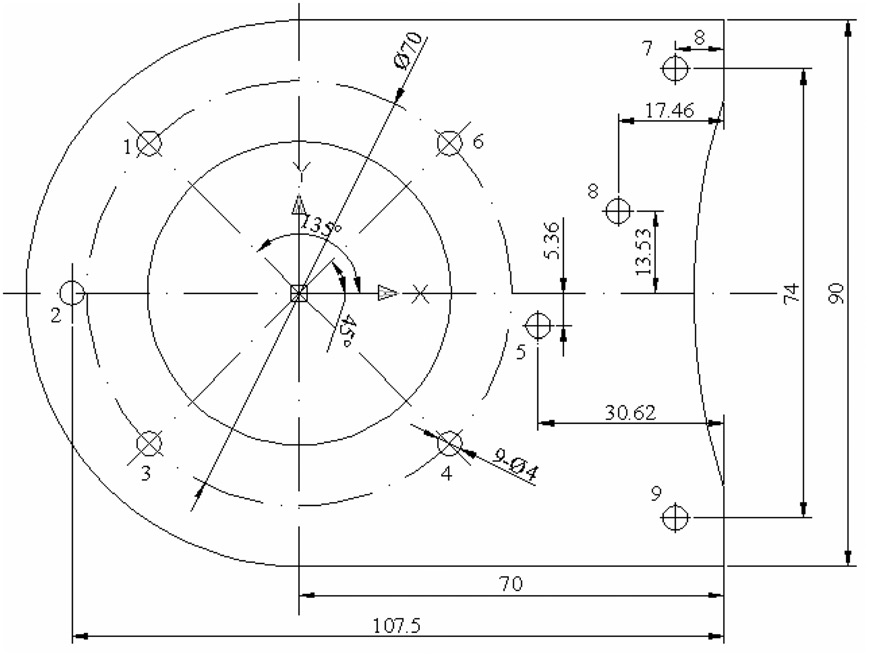
\includegraphics[width=0.45\textwidth]{figures/drilling_1.png}
        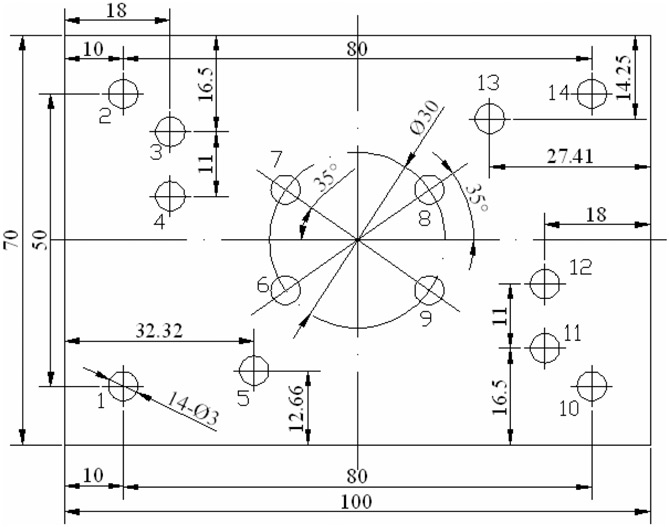
\includegraphics[width=0.45\textwidth]{figures/drilling_2.png}
        \caption{Printed circuit boards with holes to drill \cite{zhu2008drilling}}
        \label{fig:drillings}
    \end{figure}

    Zhu's paper reviews related work, including the Hopfield algorithm, evolutionary ant colony algorithm, genetic algorithm, tabu search, simulated annealing, etc.
    It follows that the drilling path problem can be expressed as a single-objective TSP.
    Hence, the particle swarm optimization (PSO) can be used.
    However, standard PSO suffers in the drilling path problem for its slow convergence.
    In their work, they propose a mechanism that comes with global convergence capability.
    This is their major contribution in this paper. 

    \subsection{Standard PSO}
    {
        In the standard PSO, the position of a particle is corresponding to a solution of the problem.
        Here in the drilling path problem, the position is encoded into a discrete space.
        Similar to TSP, the encoded space is the permutations of an integer series indicating the order that the cutting tool should follow.

        The PSO is a swarm intelligence algorithm inspired by bird swarm seeking food. 
        A swarm of particles, like birds, are moving in the search space to find a optimal location, like the food.
        The fitness value in each location, defined by the target function value, indicates the ``distance'' of the current location.
        For the $i$-th particle at time $t+1$, it has a velocity of 
        $$v_i(t+1) = [c_1 \otimes (p_i(t) - x_i(t))] \oplus [c_2 \otimes (p_g(t) - x_i(t))],$$
        where $x_i(t)$ is its current location at time $t$, 
        $p_i(t)$ is the best location the particle has searched so far, 
        and $p_g(t)$ is the best location the swarm has searched so far.
        The velocity is a linear combination, taking both individual and collective information into account.
        It follows that the location is updated according to the speed:
        $$x_i(t+1) = x_i(t) + v_i(t+1).$$

        The convergence of standard PSO has been studied by Solis and Wets (1981). 
        Their work shows that the standard PSO is not guaranteed to be a local optimization solution, nor is the local convergence.
    }

    \subsection{PSO with global convergence characteristics}
    {
        In the topical paper \cite{zhu2008drilling}, there are two key improvements:

        \subsubsection{Improvement 1}
        {
            In standard PSO, the velocity of particle $i$ at time $t+1$ should be
            $$v_i(t+1) = [c_1 \otimes (p_i(t) - x_i(t))] \oplus [c_2 \otimes (p_g(t) - x_i(t))],$$
            which does not depend on the previous speed $v_i(t)$.
        
            In the topical paper, the term of previous speed and the speed memory remain, indicating that the capability of convergence on global solution is not affected.
            $$v_i(t+1) = (\omega \otimes v_i(t)) \oplus [c_1 \otimes (p_i(t) - x_i(t))] \oplus [c_2 \otimes (p_g(t) - x_i(t))].$$
            This is probably inspired by the momentum term, or inertia term, that has been in widespread use in other algorithms such as gradient descent.
            The inertia term helps make the velocity term smoother and increase the chance of getting rid of local minimum areas by exploration.
        }

        \subsubsection{Improvement 2}
        {
            When the swarm evolves to certain generation, 
            there is at least one particle located in the best previous position of the swarm and this particle will stop evolving. 
            Then, the particle is improved by the following method to reinforce the global convergence of the algorithm.

            For the $j$-th particle at time step $t$, when the three positions of the particle $x_j(t)$, $p_j(t)$, $p_g(t)$ are superposing, the $j$-th particle will stop evolving. 
            In order to improve the convergence of the algorithm, $p_g(t)$ is kept as the best previous position of the particle swarm, 
            the $j$-th particle position $x_j(t+1)$ is generated randomly again in the search space $S$, then update $p_j(t+1)$, 
            positions of other particles $i$ can be obtained by using equations of standard PSO at time step $t+1$, then update $p_g(t+1)$.
        }

        \subsubsection{Why these improvements work}
        {
            With the improvements above, there is at least one particle $j$ whose positions $x_j(t)$, $p_j(t)$ and $p_g(t)$ are superposing in certain evolutional generations. 
            Thus at least one particle needs to be generated randomly again in the search space $S$, so the global convergence capability of the new algorithm is reinforced as a consequence.
        }
    }

}

\bibliographystyle{ieeetran}
\bibliography{reference}
\end{document}